%
\documentclass[12pt]{article}

% The usual packages
\usepackage{fullpage}
\usepackage{breakcites}
\usepackage{setspace}
\usepackage{endnotes}
%\usepackage{float} % can't use with floatrow
\usepackage{amsmath}
\usepackage{amsfonts}
\usepackage{amssymb}
\usepackage{rotating}
\usepackage{longtable}
\usepackage{microtype}
\usepackage{graphicx}
\usepackage{hyperref}
%\usepackage[usenames,dvipsnames]{color}
\usepackage{url}
\usepackage{natbib}
\usepackage{framed} 
\usepackage{epigraph}
\usepackage{lipsum}
\usepackage{enumerate}
%\usepackage{dcolumn}
%\restylefloat{table}
\bibpunct{(}{)}{;}{a}{}{,}

% Set paragraph spacing the way I like
\parskip=0pt
\parindent=20pt

%\usepackage{helvet}
\usepackage[labelfont={bf}, margin=0cm, font=small, skip=0pt]{caption}


% Define mathematical results
\newtheorem{lemma}{Lemma}
\newtheorem{proposition}{Proposition}
\newtheorem{theorem}{Theorem}
\newtheorem{claim}{Claim}
\newenvironment{proof}[1][Proof]{\begin{trivlist}
\item[\hskip \labelsep {\bfseries #1}]}{\end{trivlist}}
\newenvironment{definition}[1][Definition]{\begin{trivlist}
\item[\hskip \labelsep {\bfseries #1}]}{\end{trivlist}}
\newenvironment{example}[1][Example]{\begin{trivlist}
\item[\hskip \labelsep {\bfseries #1}]}{\end{trivlist}}
\newenvironment{remark}[1][Remark]{\begin{trivlist}
\item[\hskip \labelsep {\bfseries #1}]}{\end{trivlist}}
\DeclareMathOperator*{\argmin}{arg\,min}
\DeclareMathOperator{\med}{med}


% Set up fonts the way I like
\usepackage{tgpagella}
\usepackage[T1]{fontenc}
\usepackage[bitstream-charter]{mathdesign}

%% Baskervald
%\usepackage[lf]{Baskervaldx} % lining figures
%\usepackage[bigdelims,vvarbb]{newtxmath} % math italic letters from Nimbus Roman
%\usepackage[cal=boondoxo]{mathalfa} % mathcal from STIX, unslanted a bit
%\renewcommand*\oldstylenums[1]{\textosf{#1}}

%\usepackage[T1]{fontenc}
%\usepackage{newtxtext,newtxmath}

% A special command to create line break in table cells
\newcommand{\specialcell}[2][c]{%
 \begin{tabular}[#1]{@{}c@{}}#2\end{tabular}}


%% Set up lists the way I like
% Redefine the first level
\renewcommand{\theenumi}{\arabic{enumi}.}
\renewcommand{\labelenumi}{\theenumi}
% Redefine the second level
\renewcommand{\theenumii}{\alph{enumii}.}
\renewcommand{\labelenumii}{\theenumii}
% Redefine the third level
\renewcommand{\theenumiii}{\roman{enumiii}.}
\renewcommand{\labelenumiii}{\theenumiii}
% Redefine the fourth level
\renewcommand{\theenumiv}{\Alph{enumiv}.}
\renewcommand{\labelenumiv}{\theenumiv}
% Eliminate spacing around lists
\usepackage{enumitem}
\setlist{nolistsep}

% Create footnote command so that my name
% has an asterisk rather than a one.
\long\def\symbolfootnote[#1]#2{\begingroup%
\def\thefootnote{\fnsymbol{footnote}}\footnote[#1]{#2}\endgroup}

% Create the colors I want
\usepackage{color}
\definecolor{darkred}{RGB}{100,0,0}

\hypersetup{
pdftitle={When BLUE Is Not Best}, % title
pdfauthor={Dan K. Baissa and Carlisle Rainey}, % author
pdfkeywords={robust linear regression} {outliers} {leverage}
pdfnewwindow=true, % links in new window
colorlinks=true, % false: boxed links; true: colored links
linkcolor=black, % color of internal links
citecolor=black, % color of links to bibliography
filecolor=black, % color of file links
urlcolor=blue % color of external links
}

% section headers
%\usepackage[scaled]{helvet}
%\renewcommand\familydefault{\sfdefault} 
%\usepackage[T1]{fontenc}
%\usepackage{titlesec}
%\titleformat{\section}
%  {\normalfont\sffamily\Large\bfseries}
%  {\thesection}{1em}{}
%\titleformat{\subsection}
%  {\normalfont\sffamily\large\bfseries}
%  {\thesection}{1em}{}
%  \titleformat{\subsubsection}
%  {\normalfont\sffamily\bfseries}
%  {\thesection}{1em}{}

% enable comments in pdf
\newcommand{\dtk}[1]{\textcolor{blue}{#1}}
\newcommand{\ctk}[1]{\textcolor{red}{#1}}


\begin{document}

\begin{center}
{\LARGE \textbf{When BLUE Is Not Best}}\\\vspace{2mm}
{ \textbf{Non-Normal Errors and the Linear Model}\symbolfootnote[1]{We thank Bill Clark and Matt Golder for making their data available to us. The analyses presented here were conducted with \texttt{R} 3.2.2. All data and computer code necessary for replication are available at \href{https://github.com/carlislerainey/heavy-tails}{
github.com/carlislerainey/heavy-tails}.}}\\\vspace{2mm}


\vspace{10mm}

Daniel K. Baissa\symbolfootnote[2]{Daniel K. Baissa is a Ph.D. student in the Department of Government, Harvard University, 1737 Cambridge St., Cambridge , MA, 02138 (\href{mailto:dbaissa@g.harvard.edu}{dbaissa@g.harvard.edu}).}

\vspace{3mm}

Carlisle Rainey\symbolfootnote[3]{Carlisle Rainey is Assistant Professor of Political Science, Texas A\&M University, 2010 Allen Building, College Station, TX, 77843 (\href{mailto:crainey@tamu.edu}{crainey@tamu.edu}).}
\end{center}

\vspace{10mm}

% Abstract
{\centerline{\textbf{Abstract}}}
\begin{quote}\noindent
Researchers in political science often estimate linear models of continuous outcomes using least squares. 
While it is well-known that least-squares estimates are often sensitive to single, unusual data points, this knowledge has not led to careful practices when using least-squares estimators. 
We highlight the importance of using more robust estimators along with variable transformations and discuss several approaches to detect, summarize, and communicate the influence of particular data points. 
We conclude with a reanalysis of \cite{ClarkGolder2006} and show that the residuals are highly non-normal under their model specification. 
We show that applying an empirically-chosen transformation and/or using a robust estimator allows us to improve and extend their analysis in important ways.
 \end{quote}

% Add quote to first page
% \epigraph{}

%\begin{center}
%Manuscript word count: 
%\end{center}

% Remove page number from first page
\thispagestyle{empty}

% Start main text
\newpage
\doublespace

\section*{Introduction}

Linear models of the form $y_i = X_i\beta + \epsilon_i$ estimated with least squares remain one of the most common statistical tools in political science research \citep{KruegerLewisBeck2008}. 
Yet there seems to remain some confusion about the conditions under which least squares serves as a good estimator of the linear model. 
After assuming that the model $y_i = X_i\beta + \epsilon_i$ is correct and that the matrix $X$ is full rank, we need to make further assumptions about the errors $\epsilon_i$ to obtain desirable properties for the least-squares estimator. We might use some of the following assumptions:
\begin{enumerate}[label= A\arabic*:]
  \item Errors have mean equal to zero.
  \item Errors have a constant, finite variance.
  \item Errors are independent.
  \item Errors follow a normal distribution.
\end{enumerate}
By assuming only A1, we obtain an unbiased, consistent estimator (e.g., \citealt{Wooldridge2013}, p. 810 and pp. 385, 815-816). 
However, by assuming A1, A2, A3, and A4, we obtain the best unbiased estimator (BUE), which has the smallest possible variance among the class of unbiased estimators (e.g., \citealt{Wooldridge2013}, pp. 809-815).
 By the Gauss-Markov theorem, we can remove A4---the assumption of normal errors---and still obtain the best \textit{linear} unbiased estimator (BLUE), which has the smallest possible variance among the class of unbiased, \textit{linear} estimators (e.g., \citealt{Wooldridge2013}, pp. 809-812). 
Researchers have primarily justified least squares using the Gauss-Markov theorem because it seems to impart desirable properties without the overly restrictive assumption of normal errors.
For example, \cite{BerryFeldman1985} write: 
\begin{quote}
[The assumption of normally distributed error term] is necessary \textit{only} for tests of significance; its violation will have no effect on the estimation of the parameters of the regression model. It is quite fortunate that normality is not required for estimation, because it is often very difficult to defend this assumption in practice.
\end{quote}
\citet[p. 101]{Wooldridge2013} writes that the Gauss-Markov theorem ``justifies the use of the OLS method rather than using a variety of competing estimators.''

However, notice that a tradeoff occurs when relaxing the assumption of normal errors. 
In order to relax the assumption of normal errors (and keep desirable small sample properties), we must restrict ourselves to linear estimators. 
This raises a critical, but often overlooked question: Under what conditions can a researcher safely restrict herself to linear estimators? 
We argue that a restriction to linear estimators makes sense only when the errors follow a normal distribution. 
If the errors do not follow a normal distribution, then least-squares is still a best \textit{linear} unbiased estimator, but other, non-linear estimators may be more more efficient.
Our claim is that the restriction to linear estimators is artificial and can only be justified by assuming normal errors---an assumption that \cite{BerryFeldman1985} note is very difficult to defend in practice.

The Gauss-Markov theorem has convinced researchers in political science that as long as A1, A2, and A3---the Gauss-Markov assumptions---are met, the distribution of the errors is unimportant. 
But the distribution of the errors is crucial to a linear regression analysis.
Deviations from normality, especially large deviations commonly found in regression models in political science, can devastate the performance of least squares compared alternative estimators. 

In this paper, we emphasize the importance of errors and residuals from a statistical and substantive perspective. We adopt and defend a skeptical perspective toward least squares in favor of more robust estimators. We proceed as follows: we (1) clarify the crucial distinction between a linear \textit{model} and a linear \textit{estimator}, (2) explain that the BLUE estimator is not the best estimator unless the errors are normally distributed, (3) highlight powerful, robust alternatives to least-squares estimators that are unbiased and more efficient for a wide range of substantively plausible error distributions, (4) provide concrete, practical advice to substantive researchers using linear models, and (5) provide a compelling example that illustrates the importance of robust estimators.

\section*{Is a BLUE Estimator the Best Estimator?}

The linear model can be written as $y = X\beta + \epsilon$.\footnote{As usual, $y$ is an outcome variable of interest (usually roughly continuous), $X$ is a $n \times (k + 1)$ matrix containing a single column of ones and $k$ columns holding $k$ explanatory variables, $\beta$ is a $(k + 1) \times 1$ matrix of model coefficients, and $\epsilon$ is an $n \times 1$ matrix of errors. As usual, the statistical properties of these estimators depend on this model being correct and a full rank $X$.} 
Researchers in political science commonly estimate this model with least squares by minimizing the sum of the squared residuals, such that $\hat{\beta}^{ls} = \argmin_b S(b)$, where $S(b) = \sum_{i = 1}^n(y_i - X_ib)^2$. 
If we assume that the errors $\epsilon$ follow independent and identical normal distributions with mean zero and unknown variance, which we refer to as a ``normal-linear model,'' then the least squares estimator is the best (i.e., uniform minimum variance) unbiased estimator (BUE) (\citealt[pp. 334-342]{CasellaBerger2002}, and \citealt[807-815]{Wooldridge2013}), sometimes called the best unbiased estimator (BUE).
This is a powerful result. 
Under the assumption of normally distributed errors, least squares is the most efficient unbiased estimator.

If we relax the assumption of normality, and simply require that the errors have mean zero and constant variance, then the Gauss-Markov Theorem guarantees that the least-squares estimator is the best \textit{linear} unbiased estimator. 
While this result is often emphasized, it should provide little comfort to researchers because there is little statistical or substantive reason to restrict themselves to \textit{linear} estimators.

At first glance, one might take the linearity restriction in the Gauss-Markov theorem to refer to the structure of the model (i.e., ``linear in the parameters''). 
Indeed, this is the sense in which we use ``linear'' in the phrase ``linear model.'' 
However, the ``linear'' restriction in the Gauss-Markov Theorem refers something else---a linear \textit{estimator}, which is a technical condition that has little connection to the substance of the problem.
Linearity of the \textit{estimator} simply requires that the estimates be a linear function of the outcome variable, so that $\hat{\beta}_j = \lambda_1 y_1 + \lambda_2 y_2 + ... + \lambda_n y_n$, where the weights $\lambda_i$ are allowed to depend on $X$, but not on $y$. 
In other words, the Gauss-Markov theorem assumes a linear \textit{model} of the form $E(y | X) = X\beta$, but it also restricts researchers to linear \textit{estimators} of the form $\hat{\beta}_j = \lambda_1 y_1 + \lambda_2 y_2 + ... \lambda_n y_n$. 

We can see that the least-squares criterion produces a linear estimator with some simple algebra. 
First, recall that we wish to minimize $S(b) = \sum_{i = 1}^n(y_i - X_ib)^2$ with respect to $b$. 
To do this, we can simply set $\dfrac{\partial S(\hat{\beta}^{ls})}{\partial \hat{\beta}^{ls}} = 0$ and solve for the vector $\hat{\beta}^{ls}$. 
Noting that $\dfrac{\partial S(\hat{\beta}^{ls})}{\partial \hat{\beta}^{ls}} = \sum_{i = 1}^n 2(y_i - X_i\hat{\beta}^{ls})(-X_i) = 0$ implies that $\sum_{i = 1}^n X_i(y_i - X_i\hat{\beta}^{ls}) = 0$. 
This is simply a system of $k+1$ \textit{linear} equations $\sum_{i = 1}^n X_{ij}(y_i - X_i\hat{\beta}^{ls})$ for $k = \{0, 1, 2,..., k\}$. 
Of course, the matrix form $X'(y - X\hat{\beta}^{ls}) = 0 \Rightarrow (X'X)\hat{\beta}^{ls} = X'y \Rightarrow \hat{\beta}^{ls} = (X'X)^{-1}X'y$ is much more common. 
In matrix form, linearity of the estimator requires that $\hat{\beta} = My$, where $M$ depends on the matrix $X$. 
We can clearly see that the least squares estimator $\hat{\beta}^{ls} = (X'X)^{-1}X'y$ has the form $My$.

However, restricting ourselves to linear estimators is neither necessary nor productive. 
Note that we are not arguing against linear models (i.e., linear in the parameters), such as 
\begin{align*}
y_i &= \beta_0 + \beta_1\log(x_i) + \epsilon_i\text{,}\\
y_i &= \beta_0 + \beta_1x_i + \beta_2x_i^2 + \epsilon_i\text{, or}\\ 
y_i &= \beta_0 + \beta_1x_i + \beta_2z_i + \beta_3x_iz_i + \epsilon_i\textit{.}
\end{align*}
This collection of linear models illustrates that the linear model can represent a wide range of theoretically-relevant relationships, especially when it includes explanatory variables non-linearly. 
But there is no statistical reason to restrict ourselves to linear \textit{estimators} for these linear models, except for mathematical convenience and computational ease.
The only substantive reason to restrict ourselves to linear estimators is if we are willing to assume that we have normally distributed errors. 
Under this assumption, linearity is a reasonable restriction---indeed, the linear estimator is the BUE when the errors are normal.
Restriction to linearity does not get us away from the assumption of normality because BLUE estimators are BUE estimators only under the assumption of normal errors.
If the errors are not normally distributed, then the one can easily better the BLUE estimator.

%But we might also make a substantive argument \textit{against} linear estimators (i.e., weighting all observations equally). 
%We suggest two potentially desirable properties of estimators. 
%First, we might prefer estimators that provide an excellent fit to \textit{most} of the data rather rather than a mediocre fit to \textit{all} the data. 
%Secondly, we might prefer an estimate that treats unusual data equally---as inconsistent the the model.
%Neither of these behaviors is possible with linear estimators.
%
%For example, consider the estimates shown in the left panel of Figure \ref{fig:best-fit-illustration}. 
%Which of the two estimates, A or B, best summarizes the relationship between the explanatory and outcome variable? 
%Estimate A fits all the data reasonably well, but estimate B provides an excellent summary for most of the data. 
%Which is preferred? 
%At least in some cases, we might prefer estimate B because we wish to discount the three unusual cases as inconsistent with the model (perhaps these cases are elections marred with scandals, etc.).
%
%\begin{figure}[h!]
%\begin{center}
%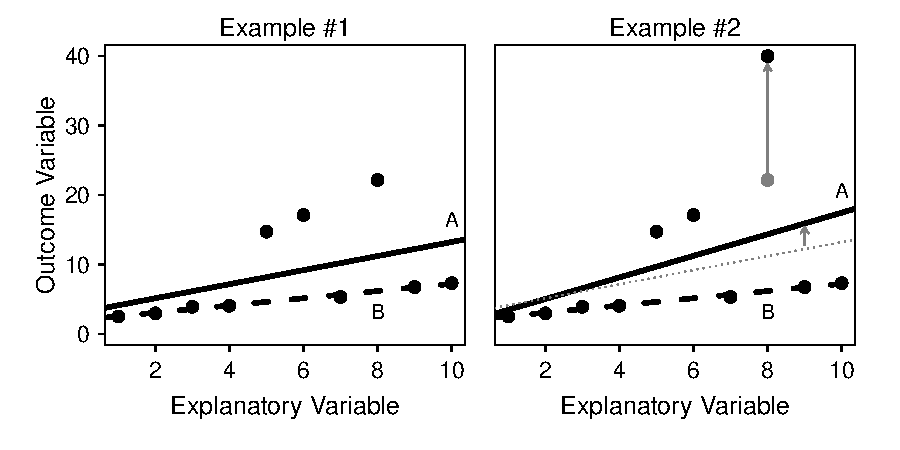
\includegraphics[scale = .7]{figs/best-fit-illustration.pdf}
%\caption{This figure shows to hypothetical examples that illustrate two potentially desirable properties of estimators.
%The left panel illustrates that one estimator (A) might provide an excellent fit to most of the data while another estimator (B) might provide a mediocre fit to all the data. 
%The right panel illustrates that one estimator (A) might ignore changes among the unusual cases while anther estimator (B) might be quite responsive.}\label{fig:best-fit-illustration}
%\end{center}
%\end{figure}
%
%Secondly, we might prefer an estimator that gives zero weight to cases that fall outside the explanatory power of the model.
%These cases seem somehow different and we might prefer that these unusual data to not degrade the excellent fit for the majority of the data. 
%That is, if one unusual case becomes \textit{even more} unusual, the estimates should not change. 
%Stated differently, we might prefer an estimator that \textit{ignores} changes in the unusual cases, such as estimator B in the right panel of Figure \ref{fig:best-fit-illustration}, over an estimator that \textit{resonds to} changes in the unusal cases, such as estimator A in the right panel of Figure \ref{fig:best-fit-illustration}.
%
%Even if one does not to use an estimator with either of these behaviors, then following example illustrates the artificiality of the linearity restriction. 
If the researcher has a substantive or empirical reason to assume a non-normal distribution for the errors, such as a slightly heavier-tailed $t_{10}$ distribution, then the linear restriction in the Gauss-Markov theorem prohibits comparisons to the more efficient (but non-linear) MLE estimator implied by the assumed $t_{10}$ error distribution. 
Similarly, the linear restriction prohibits comparisons to the least absolute deviation estimator, which the is the MLE and is more efficient than least squares when the errors follow a Laplace distribution. 

It is not often appreciated, at least in practice, that if the errors do not follow independent and identical normal distributions, then the least squares is no longer the BUE---other well-understood and easily computed estimators might outperform least squares. 
Indeed, for some error distributions, least squares might perform substantially worse.

Many researchers simply assume a normal-linear model for little or no substantive or empirical reason. 
Even while knowing that the assumed normal-linear model is \textit{in}correct, researchers use this model as an approximation. 
But if the model is only an approximation, then the desirable statistical properties are not longer guaranteed (e.g., unbiasedness, minimum variance). 
With this in mind, it makes more sense to use a robust estimator with the following qualitative properties in typical sample sizes:
\begin{enumerate}
\item When the normal-linear model is exactly correct, the estimator should be approximately unbiased with efficiency comparable to, but less than, least squares.
\item When the deviation from the normal-linear model is small, the estimator should be approximately unbiased with efficiency comparable to, but perhaps greater than, least squares.
\item When the deviation from the normal-linear model is large, the estimator should exhibit relatively little bias and be much more efficient than least squares.
\end{enumerate}
\noindent The ``best'' model for a social scientist might not be the optimal estimator for an assumed model, but an estimator that works reasonably well for the assumed model and many substantively plausible deviations. 

To see the importance of this in practice, we simulated 10,000 data sets 50 observations of variables $x$ and $y$, where the relationship between $x$ and $y$ is given by $y = x + \epsilon$, where $\epsilon$ follows a $t$ distribution with three degrees of freedom. 
Note that the $t_3$ distribution is symmetric, bell-shaped, and resembles the normal distribution, except it has heavier tails. 
For each of these 10,000 data sets, we used least-squares to estimate the slope of the relationship between $x$ and $y$, where the true value equals one. 
Because we simulated these data, we know that the Gauss-Markov assumptions hold. 
This means that least squares is the \textit{best} linear unbiased estimator. 
The left panel of Figure \ref{fig:lts-illustration} shows the distribution of the estimated slopes using least squares.

\begin{figure}[h!]
\begin{center}
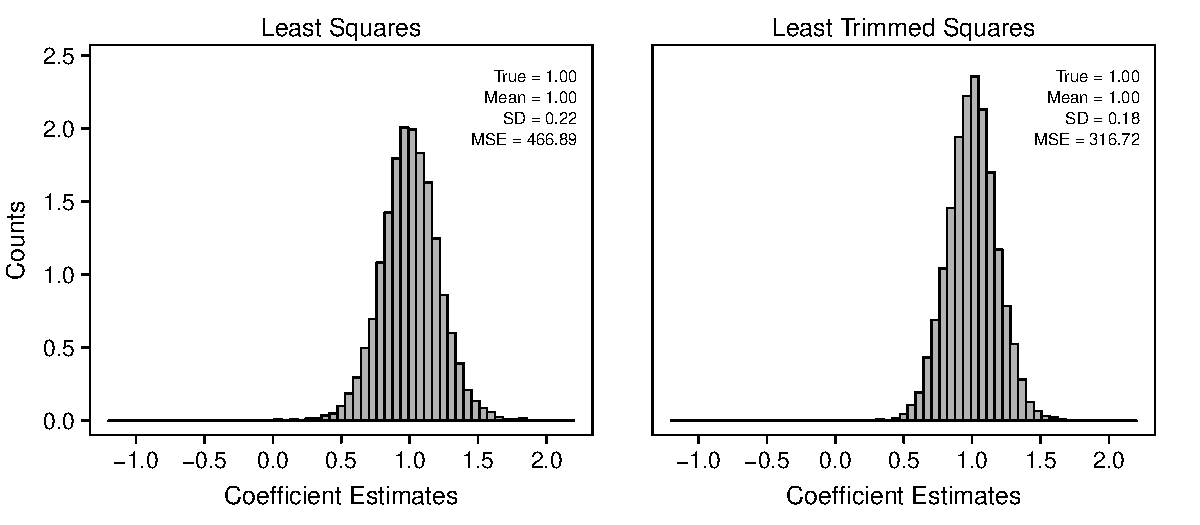
\includegraphics[scale = .7]{figs/lts-illustration.pdf}
\caption{These two histograms show the sampling distribution for the least squares estimator and the least trimmed squares estimator under the true model $y = x + \epsilon$, where $\epsilon \sim t_3$. 
Notice that despite least squares being the best linear unbiased estimator for the problem, the least trimmed squares estimator is a better estimator.}\label{fig:lts-illustration}
\end{center}
\end{figure}

But we also consider a least trimmed squares (LTS) estimator in which we minimize the smallest 90\% of the residuals. 
This method literally throws away data. 
Though it lacks the elegant theory of the least squares estimator, the right panel of Figure \ref{fig:lts-illustration} shows that it is unbiased and more efficient that the least-squares estimator. 
The standard deviation of the estimates from the LTS estimator is about about 18\% smaller than the BLUE estimator, and the mean squared error is about 32\% smaller. 
By any reasonable standard, the LTS estimator is a better estimator than the least squares estimator in this example, yet the least squares estimator is BLUE. 
We obtain this improvement by expanding our focus to non-linear estimators, such as the LTS estimator. 
In this case, the LTS estimator is non-linear because it places zero weight on the largest 10\% of the residuals and weights of one on the smallest 90\% of the residuals.

\section*{The Relative Emphasis on Standard Errors}

There has been a great deal of attention in the methodological literature to the sensitivity of standard errors to violations from the assumed model---and substantive scholars have paid attention.
White's (\citeyear{White1980}) seminal paper developing heteroskedasticity-consistent standard errors has received over 20,000 citations, making it one of the most cited papers in economics.
Beck and Katz's (\citeyear{BeckKatz1995}) development panel corrected standard errors has received over 4,300 citations, making it one of the most cited papers in political science.

On the other hand, there has been scant attention paid by substantive political scientists to the sensitivity of the \textit{estimates} to similar violations. 
This is particularly problematic, since it makes little sense to find a good standard error for a poor estimate (\citealt{Freedman2006} and \citealt{KingRoberts2014}). 
Two papers in political science have addressed the issue of robust estimation. 
\cite{Western1995} introduces political scientists to robust estimators, but this work has been essentially ignored. 
Although it is more broadly applicable than \cite{BeckKatz1995} and was published in the same year, but it has received only 99 citations, or  about 2\% of the citations that Beck and Katz have received. 
Similarly, \cite{HardenDesmarais2011} have received only one citation, and it comes from the authors themselves.
Anderson's (\citeyear{Anderson2008}) broad and accessible introduction to robust estimation methods has received only about 150 citations, most from outside political science.

This focus on obtaining reasonable standard errors at the expense of reasonable estimates can be seen in \cite{Gujarati2004}. Though the text deals with robust standard errors in some detail, \citet[p. 339]{Gujarati2004} writes in a footnote:
\begin{quote}
In passing, note that the effects of departure from normality and related topics are often discussed under the topic of robust estimation in the literature, a topic \textit{beyond the scope of this book} [italics ours].
\end{quote}
\cite{AngristPischke2009} devote an entire chapter to robust standard errors and completely ignore robust estimation of model coefficients. 
\cite{Wooldridge2013} does devote about two pages to robust estimation, though the tone is skeptical.

\section*{Dealing with Skewness: Transforming the Outcome}

Despite the lack of attention devoted by substantive scholars to non-normal errors, there are two ways in which the errors can deviate from normality, and both negatively affect inferences when using least squares. 
\begin{enumerate}
\item The error distribution might be skewed. 
\item The error distribution might have heavy tails. 
\end{enumerate}

We suggest dealing with these two deviations differently, so we discuss each separately.

Skewed error distributions create two problems for the linear model. 
First, least squares estimates the quantity $E(Y | X)$ and the mean is not a good summary of location for skewed variables. 
Symmetric error distributions are easier to understand. 

Second, and perhaps most importantly, skewed error distributions indicate a lack of model fit. 
It is sometimes theoretically intuitive to believe that the explanatory variables should have increasing effects non-negative outcome variables, such as an individual's annual income. 
Rather than a college degree increasing one's expected income by \$10,000, perhaps a college degree increases it by 10\%. 
If this intuition is correct and a researcher relies on the statistical model $\text{Income}_i = \beta_0 + \beta_1 \text{College Degree}_i + \epsilon_i$, then the errors will have a strong skew to the right. Simply logging the outcome, or using the model $\log (\text{Income}_i) = \beta_0 + \beta_1 \text{College Degree}_i + \epsilon_i$, better captures the theoretical intuition.

Even if we remain indifferent toward the theoretical implications of skewed error distributions, we must remain cautious about the statistical implications. 
Indeed, the log-transformation in the example above improves the efficiency of the least squares estimator by making the assumption of normally-distributed errors more appropriate (not to mention the linearity of the model).
The performance of least squares estimators improves as the error distribution approaches a normal distribution. 

It is quite common in disciplines such as economics, for example, to log-transform non-negative outcome variables by default. 
Since non-negative (or strictly positive) outcomes are bounded below by zero, then these variables are likely skewed to the right---they are squeezed from the left by zero. 
In this case, the model $\log(y) = X\beta + \epsilon$ will likely provide a better approximation to the data.

When handling skewed residuals, it is impossible to know whether (1) the skew is due to a misspecification of the outcome variable (i.e., failing to transform) or (2) the errors simply follow a heteroskedastic, skewed distribution. 
However, we can be confident that heavily skewed residuals are \underline{in}consistent with the normal errors---the researcher must do something to address the skew.
Transforming the outcome variable is one effective method for making the model more consistent with the data.

\subsection*{The Box-Cox Transformation}

While we agree with the spirit of the suggestion to log-transform non-negative outcome variable $y$, statisticians have created more precise empirical methods for choosing \textit{whether} and \textit{how} to do the transformation. 
\cite{BoxCox1964} propose the Box-Cox transformation 
\begin{displaymath}
   y^{(\lambda)} = BC(y, \lambda) = \left\{
     \begin{array}{lr}
       \dfrac{y^\lambda - 1}{\lambda} & \text{for } \lambda \neq 0\\
       \log y & \text{for } \lambda = 0
     \end{array}
   \right.,
\end{displaymath}
\noindent where the transformation parameter $\lambda$ is estimated with maximum likelihood. 
In this case, the model becomes $y^{(\lambda)} = X\beta + \epsilon$. 
This is particularly convenient because $\hat{\lambda} \approx 1$ suggests no transformation is needed and $\hat{\lambda} \approx 0$ suggests that only an intuitive log-transformation is needed.

Researchers can easily assess the skewness in the residuals using a simple histogram of the residuals or a QQ plot of the residuals compared to their normal quantiles. 
For a formal test of skewness, researchers might use a direct test for symmetry on residuals $\hat{e}$, such as the Mira test \citep{Mira1999} or simply test whether $\lambda \neq 1$ under the Box-Cox framework. 
However, we do not want to argue for a particular test, but to highlight that (1) asymmetries worsen the performance of least squares and many robust methods, (2) researchers can easily detect asymmetries by carefully examining the residuals, and (3) researchers can address this problem with simple, easy-to-use transformations.

\subsection*{Mean or Median?}

Applying a non-linear transformation to the outcome variable $y$ does raise an interpretational difficulty. 
The usual, untransformed linear model is given by $y = X\beta + \epsilon$ and the quantity of interest is usually $E(y | X)$ or $\frac{\partial E(y | X)}{\partial x_j}$. 
For concreteness, consider the log-transformation. 
Using the same logic, then the model is $log(y) = X\beta + \epsilon$ and we might take the quantity of interest to be $E[\log(y) | X]$ or $\frac{\partial E[\log(y) | X]}{\partial x_j}$. 
However, the substantive researcher is usually interested in $y$, not $\log(y)$, making $\frac{\partial E[\log(y) | X]}{\partial x_j}$ more difficult to understand than $\frac{\partial E(y | X)}{\partial x_j}$. 
To make the results more interpretable, we simply need to ``undo'' the transformation. 
But $E[\log(y) | X] \neq \log [E(y | X)]$, which means that the log cannot simply be undone without additional computation.

These interpretational difficulties are not due to the choice to transform the data, but imbedded in the data themselves. 
In the context of skewed distributions, the mean $E(\cdot)$ is not a good summary of the ``center'' of the data. 
While the mean often makes calculations easier, the median offers a better summary of location. 
The median also has an intuitive interpretation because one-half of the distribution lies above the median and one-half lies below. 
If a researcher uses $\med(y_{new} | X_{new})$ to predict the unknown outcome $y_{new}$ for a known case $X_{new}$, then she has a 50\% chance of being too high and a 50\% chance of being too low. 

In addition to the intuitive substantive interpretation of $\med(y | X)$, the median has another desirable property. 
Because the log-transformation is order-preserving, $\med[\log(y) | X] = \log [\med(y | X)]$, which means that the log \textit{can} easily be undone because $e^{\med[\log(y) | X]} = e^{\log[\med(y | X)]} = \med(y | X)$. 
Therefore, by adopting $\med(y | X)$ and $\frac{\partial \med(y | X)}{\partial x_j}$ as the quantities of interest, the researcher eases the interpretation of the results and can easily move between transformed and untransformed outcomes (e.g., $\med[\log(y)] \rightarrow \med(y)$). 
This holds for the more general case of $y^{(\lambda)}$ as well.

\subsection*{Simulating Quantities of Interest Under Transformation}

To obtain quantities of interest relating to $\med(y)$ when the estimated model has the generic form $y^{(\lambda)} = X\beta + \epsilon$, one can simply use the algorithm described in \cite{KingTomzWittenberg2000}.
\begin{enumerate}
\item Estimate the Box-Cox transformation parameter $\hat{\lambda}$ using maximum likelihood. 
(If the values one or zero fall within the confidence interval, then one may wish to use those values to maintain the direct interpretability of the model coefficients.)
\item Estimate the transformed model $y^{(\hat{\lambda})} = X\beta_{trans} + \epsilon$ and obtain the estimated model coefficients $\hat{\beta}_{trans}$ and covariance matrix $\Sigma_{trans}$.
\item Choose a hypothetical case or set of cases $X_{pred}$ for which to calculate the quantity of interest. 
If one is interested in calculating a first difference, it is convenient to use $X_{hi}$ and $X_{lo}$, where the first-difference $\Delta(y, X_{hi}, X_{lo}) = \med(y | X_{hi}) - \med(y | X_{lo})$.
\item Following \cite{KingTomzWittenberg2000}, for $i$ from one to a large (e.g., 1,000) number of iterations $n_{sims}$:
        \begin{enumerate}
        \item Simulate $\tilde{\beta}_{trans} \sim N\left(\hat{\beta}_{trans}, \Sigma_{trans}\right)$.
        \item If interested in the predicted value, then calculate and store $\tilde{Q}_i = \med(y | X_{pred}, \tilde{\beta}_{trans}) = BC^{-1}(X_{pred}\tilde{\beta}_{trans}, \hat{\lambda})$. If interested in the first-difference, the calculate and store $\tilde{Q}_i = \Delta(X_{hi}, X_{lo}, \tilde{\beta}_{trans}) = BC^{-1}(X_{hi}\tilde{\beta}_{trans}, \hat{\lambda}) - BC^{-1}(X_{lo}\tilde{\beta}_{trans}, \hat{\lambda})$.
        \end{enumerate}
\item Summarize the $n_{sims}$ simulations. 
The mean or median of $\tilde{Q}$ serves as an estimate of the quantity of interest and the standard deviation of $\tilde{Q}$ serves as an estimate of the standard error. The 5th and 95th percentiles of $\tilde{Q}$ serve as an estimate of the (likely asymmetric) 90\% confidence interval for the quantity of interest.
\end{enumerate}

\section*{Dealing with Heavy-Tails: $M$-Estimation}

In spite of the scant attention paid to robust estimators in political science, statisticians have developed and refined many robust methods since the seminal work of \cite{Box1953} and \cite{Huber1964}. 
\cite{HuberRonchetti2009} provide a detailed review of these developments and \cite{Anderson2008} provides an accessible introduction. 
Adjudicating among the many robust alternatives to least squares is beyond the scope of our paper, but, to fix ideas, we do introduce one robust estimator in detail which has several desirable properties---the $M$-estimator with Tukey's biweight function. 
However, there are many other options that are beyond the scope of this paper, such as $M$-estimators with other objective functions (e.g., \citealt{Huber1973}), LMS- and LTS-estimators \citep{Rousseeuw1984}, S-estimators \citep{RousseeuwYohai1984}, and MM-estimators \citep{Yohai1987}.

While least squares yields the coefficients that minimize the sum of the squared residuals, so that $\hat{\beta}^{ls} =\argmin_{b} \sum_{i = 1}^n (y_i - X_ib)^2$, M-estimators minimizes an arbitrary, usually less-rapidly increasing function of the residuals $\hat{\beta}^{\rho} =\argmin_{b} \sum_{i = 1}^n \rho(y_i - X_ib)$. 
The function $\rho(\cdot)$ is typically chosen to be non-negative, symmetric about zero, and decreasing away from zero. 
For example, \cite{HardenDesmarais2011} recommend the least absolute deviation (LAD) estimator \citep{Dodge1987} that such $\rho(\cdot) = \text{abs}(\cdot)$. 
However, other estimators offer better performance, particularly when the normal-linear model is approximately correct. 
In particular, we recommend Tukey's biweight function, so that
\begin{displaymath}
   \rho_{bw}(r_i) = \left\{
     \begin{array}{lr}
       \dfrac{k^2}{6}\left\{ 1 - \left[ 1 - \left( \dfrac{r_i}{k} \right)^2 \right]^3\right\} & \text{for } |r_i| \leq k\\
        \dfrac{k^2}{6} & \text{for } |r_i| > k 
\end{array}
   \right.,
\end{displaymath}
\noindent where $r_i = y_i - X_ib$ and $k$ is a tuning parameter usually set to 4.685 to ensure good performance under the normal-linear model. 
We refer to the $M$-estimator using the biweight objective function as the ``biweight (BW) estimator.'' 
The BW estimator is a compelling alternative to the LAD estimator suggested by \cite{HardenDesmarais2011} for two reasons. 
First, the biweight objective function is redescending, which means that it has the ability to weight unusual observations all the way down to zero. 
The absolute value objective function, on the other hand, does downweight unusual observations, but these always received some weight. 
Secondly, the BW estimator is much more efficient than the LAD estimator when the errors are approximately normal. 

Two cautions are in order. 
First, the optimization problem is not convex, so standard routines can produce a local rather than the global minimum. 
However, researchers can usually handle this problem in practice by using a good starting value, such as the LTS estimate. 
Second, because the solution is not scale invariant, the residuals $\hat{e_i}$ are standardized by a robust estimate of scale $\hat{\sigma}_{mad}$, which must of course be estimated jointly, so that $\hat{\beta}^{bw} =\argmin_{b} \sum_{i = 1}^n \rho_{bw}\left(\dfrac{y_i - X_ib}{\hat{\sigma}_{mad}}\right)$, where $\hat{\sigma}_{mad} = \dfrac{\med\left( |y - Xb | \right)}{0.6745}$. 
Dividing by 0.6745 makes $\hat{\sigma}_{mad}$ a consistent estimator of the standard deviation of normal distribution.

While the theory for $M$-estimators remains less complete than the theory for least squares estimators, $M$-estimators do have desirable statistical properties. 
In general, $M$-estimators are consistent as long as (1) $\rho(\cdot)$ is convex or (2) the errors follow strongly unimodal distribution (i.e., decreasing away from zero). 
Because the biweight objective function is not convex, we must assume that the errors follow a strongly unimodal distribution, which ensures that the estimates are consistent and distributed asymptotically normal.

$M$-estimators in general, and the biweight estimator in particular, have the desirable substantive property that they allow unusual cases to ``be unusual.''
Least squares, on the other hand, sacrifices fit on typical cases to better fit unusual cases. 
Allowing unusual cases to stand out, though, is extremely important because unusual cases can inform and improve subsequent analyses. 
Knowing what cases fall outside the explanatory power of the model enables the researcher to ask ``Why?'' and raise issues relating to concepts, theory, and measurement that might otherwise have been missed.

\subsection*{Estimation}

The model parameters $\hat{\beta}^{bw}$ and $\hat{\sigma}_{bw}$ can be quickly estimated jointly using the following iterative algorithm.
\begin{enumerate}
\item Start with initial estimate of the coefficients $\hat{\beta}^{(0)}$. The choice of initial estimator is not trivial. 
In the case of extreme outliers and/or many parameters, starting with least squares might lead the algorithm to a local minimum. 
We recommend using the least trimmed squares method discussed earlier to obtain starting values.
\item Extract the residuals $r^{(0)} = y - X\hat{\beta}^{(0)}$. 
Use these residuals to estimate the rescaled MAD so that $\hat{\sigma}^{(0)}_{mad} = \dfrac{\med\left( |y - X\hat{\beta}^{(0)}|\right)}{0.6745}$.
%\item Assign weights $w$ according to the function $\rho$ and denote $\text{diag}(w) = W$.
\item For $i$ from one until convergence:
        \begin{enumerate}
        \item Using $\hat{\beta}^{(i-1)}$ and $\hat{\sigma}^{(i-1)}_{mad}$ assign weights $w$ according to the function $\rho$ and denote $\text{diag}(w) = W$.
        \item Calculate $\hat{\beta}^{(i)} = (X'WX)^{-1}X'Wy$.
        \item Calculate $\hat{\sigma}^{(i)}_{mad} = \dfrac{\med\left( |y - X\hat{\beta}^{(i)}|\right)}{0.6745}$
        \item The algorithm has converged when $r^{(i-1)} \approx r^{(i)}$.
        \end{enumerate}
\end{enumerate}

If we assume that the errors are symmetricaly distributed about zero, then any objective function $\rho$ that is also symmetric about zero (including, for example, the biweight objective function) produces an unbiased estimate of the parameters. 
But this estimator is \textit{linear} if and only if $\rho(r_i) = r_i^2$. Other choices of $\rho(\cdot)$ might produce better estimators than the BLUE estimator.  

The theory for the variance for this broad class of unbiased $M$-estimators, though, is asymptotic. 
The required sample size for the asymptotic approximations to work well depends on the problem, but valid confidence intervals for small data can easily be computed by bootstrapping (\citealt{Efron1981} and \citealt{MooneyDuval1993}). 

\section*{Monte Carlo Simulations}

To understand and illustrate how the performance of the biweight (BW) estimator compares with the common least squares (LS) estimator and the least absolute deviation (LAD) estimator suggested by \cite{HardenDesmarais2011}, we simulated from the linear model $y = \beta_0 + \beta_1x_1 + \beta_2 x_2 + \beta_3 x_3 + \epsilon$, where $\beta_0 = 0$ and $\beta_1 = \beta_2 = \beta_3 = 1$ and the $x_i$'s were generated from independent standard normal distributions. 
We used four different distribution for the errors.
\begin{itemize}
\item \textit{Laplace distribution.} 
The Laplace distribution has tails that decrease exponentially, but behaves much differently from the normal distribution near zero. 
Rather than ``shoulders,'' the Laplace distribution has a sharp peak at zero and can be thought of as combining two exponential distributions, one in the positive direction and the other in the negative direction.
The LAD estimator is the maximum likelihood estimator when the errors follow a Laplace distribution.
\item \textit{$t_2$ distribution.} 
The $t$ distribution with two degrees of freedom has very heavy tails. 
Because the least squares estimator weights all points equally (conditional on $X$), the extreme outliers produced by the $t_2$ distribution makes least squares a very inefficient estimator.
\item \textit{$t_{10}$ distribution.} 
The $t$ distribution with ten degrees of freedom has \textit{slightly} heavier tails than the normal distribution. 
The $t_{10}$ and normal distributions are so similar that a Shapiro-Wilk test of normality only correctly rejects the null in about 65\% of repeated samples if 500 observation are simulated from a $t_{10}$ distribution.\footnote{One needs about 750 samples to reach 80\% power.} 
It is essentially impossible to spot the differences between the normal and $t_{10}$ density functions without plotting the two directly on top of each other.
\item \textit{Normal Distribution.} The normal distribution yields the optimal conditions for the LS estimator. 
When the errors follow a normal distribution, the LS estimator has the smallest variance of all unbiased estimators. 
\end{itemize}

For each of two different sample sizes, 100 and 1,000, and the four different error distributions, we simulated 10,000 data sets, estimated $\beta_1$ using the LS estimator, the LAD estimator, and the BW estimator. 
For each condition, we calculated the expected value of the estimate and the mean squared error (MSE). 
Table \ref{tab:mc-sims-100} provides the results for the sample size of 100 and \ref{tab:mc-sims-1000} provides the results for the sample size of 1,000. 
These results show that all three estimators are unbiased regardless of the error distribution and sample size. 
Efficiency, however, varies considerably across the estimators.


\begin{table}[h!]
{\scriptsize
% quantreg::latex.table(x = ta, file = "doc/tabs/mc-sims-100",      rowlabel = "", cgroup = c("Mean", "Standard Deviation", "Mean Squared Error"),      rgroup = c("Absolute Performance", "Relative Performance"),      n.rgroup = c(3, 2), dec = 3, table.env = FALSE, label = "tab:mc-sims-100") 
%
\begin{center}
\begin{tabular}{|l||c|c|c|c||c|c|c|c||c|c|c|c|} \hline
\multicolumn{1}{|l||}{\bf }&\multicolumn{4}{c||}{\bf Mean}&\multicolumn{4}{c||}{\bf Standard Deviation}&\multicolumn{4}{c|}{\bf Mean Squared Error}\\ \cline{2-13}
\multicolumn{1}{|l||}{}&\multicolumn{1}{c|}{Lapl.}&\multicolumn{1}{c|}{$t_2$}&\multicolumn{1}{c|}{$t_{10}$}&\multicolumn{1}{c||}{Norm.}&\multicolumn{1}{c|}{Lapl.}&\multicolumn{1}{c|}{$t_2$}&\multicolumn{1}{c|}{$t_{10}$}&\multicolumn{1}{c||}{Norm.}&\multicolumn{1}{c|}{Lapl.}&\multicolumn{1}{c|}{$t_2$}&\multicolumn{1}{c|}{$t_{10}$}&\multicolumn{1}{c|}{Norm.}\\ \hline
{\bf Absolute Performance}&&&&&&&&&&&&\\
~~Least Squares&~~~0.999&~~~1.000&~~~1.001&~~~0.999&~~~0.151&~~~0.319&~~~0.114&~~~0.099&~227.419&1016.182&~130.867&~~98.850\\ 
~~Least Absolute Deviation&~~~0.999&~~~0.999&~~~1.003&~~~1.000&~~~0.126&~~~0.146&~~~0.131&~~~0.124&~159.499&~212.360&~172.911&~154.714\\ 
~~Tukey's Biweight&~~~1.000&~~~0.999&~~~1.001&~~~0.999&~~~0.131&~~~0.138&~~~0.113&~~~0.102&~172.043&~189.519&~127.731&~104.759\\ \hline
{\bf Relative Performance}&&&&&&&&&&&&\\
~~LAD/LS&~~~1.001&~~~0.999&~~~1.002&~~~1.001&~~~0.837&~~~0.457&~~~1.149&~~~1.251&~~~0.701&~~~0.209&~~~1.321&~~~1.565\\ 
~~BW/LS&~~~1.001&~~~1.000&~~~1.000&~~~1.000&~~~0.870&~~~0.432&~~~0.988&~~~1.029&~~~0.757&~~~0.187&~~~0.976&~~~1.060\\ 
\hline
\end{tabular}
\end{center}

}
\caption{This table summarizes the Monte Carlo simulations for four different error distributions with a sample size of 100. 
Notice that the BW has the best or nearly best performance in each condition, while the LAD estimator performs quite poorly for the $t_{10}$ and normal distributions and the LS estimator performs quite poorly for the Laplace and $t_2$ distributions.}\label{tab:mc-sims-100}
\end{table}

\begin{table}[h!]
{\scriptsize
% quantreg::latex.table(x = ta, file = "doc/tabs/mc-sims-1000",      rowlabel = "", cgroup = c("Mean", "Mean Squared Error"),      rgroup = c("Absolute Performance", "Relative Performance"),      n.rgroup = c(3, 2), dec = 3, table.env = FALSE, label = "tab:mc-sims-1000") 
%
\begin{center}
\begin{tabular}{|l||c|c|c|c||c|c|c|c|} \hline
\multicolumn{1}{|l||}{\bf }&\multicolumn{4}{c||}{\bf Mean}&\multicolumn{4}{c|}{\bf Mean Squared Error}\\ \cline{2-9}
\multicolumn{1}{|l||}{}&\multicolumn{1}{c|}{Lapl.}&\multicolumn{1}{c|}{$t_2$}&\multicolumn{1}{c|}{$t_{10}$}&\multicolumn{1}{c||}{Norm.}&\multicolumn{1}{c|}{Lapl.}&\multicolumn{1}{c|}{$t_2$}&\multicolumn{1}{c|}{$t_{10}$}&\multicolumn{1}{c|}{Norm.}\\ \hline
{\bf Absolute Performance}&&&&&&&&\\
~~Least Squares&~~0.999&~~0.999&~~1.000&~~1.000&~20.173&165.585&~12.793&~~9.998\\ 
~~Least Absolute Deviation&~~1.000&~~1.000&~~1.001&~~1.000&~11.352&~19.928&~17.123&~15.867\\ 
~~Tukey's Biweight&~~0.999&~~1.000&~~1.000&~~1.000&~14.705&~18.567&~12.482&~10.523\\ \hline
{\bf Relative Performance}&&&&&&&&\\
~~LAD/LS&~~1.001&~~1.000&~~1.000&~~1.000&~~0.563&~~0.120&~~1.338&~~1.587\\ 
~~BW/LS&~~1.000&~~1.000&~~1.000&~~1.000&~~0.729&~~0.112&~~0.976&~~1.053\\ 
\hline
\end{tabular}
\end{center}

}
\caption{This table summarizes the Monte Carlo simulations identical to those in Table \ref{tab:mc-sims-100}, except with a sample size of 1,000 rather than 100. 
As with Table \ref{tab:mc-sims-100}, notice that the BW has the best or nearly best performance in each condition, while the LAD estimator performs quite poorly for the $t_{10}$ and normal distributions and the LS estimator performs quite poorly for the Laplace and $t_2$ distributions.}\label{tab:mc-sims-1000}
\end{table}

The LAD estimator is the MLE when the errors follow a Laplace distribution, so, as we might expect, the LAD performs well for Laplace errors, with a MSE about 30\% lower than the LS estimate. 
However, the BW estimator also performs quite well for the Laplace distribution, with a MSE about 25\% less than the LS estimator for $N = 100$. 
For $N = 1,000$, the results are similar. 
The MSE of the LAD estimator is about 43\% than the LS estimator and the BW estimator is about 27\% lower.

The $t_2$ distribution is nearly a worst case for the LS estimator, so both robust alternatives perform considerably better. 
For $N = 100$, the LAD estimator has a MSR about 79\% lower than the LS estimator and the BW estimator has a MSE about 81\% lower. 
For $N = 1,000$, the MSE for the LAD estimator is about 85\% lower than the LS estimator and the MSE for the BW estimator is about 86\% lower. 

The $t_{10}$ distribution is a much more interesting case, because it is very similar to a normal distribution. 
Indeed, even statistical tests have trouble distinguishing the $t_{10}$ from the normal, even with large samples (e.g., with $N = 500$, the Shapiro-Wilk test of normality has about 65\% power). 
In this case, the LAD estimator has a 34\% larger MSE than the LS estimator for $N = 100$ and about a 32\% larger MSE for $N = 1,000$. 
The BW estimator, on the other hand, shows a small \textit{improvement} over the LS estimator, with an MSE about 2\% \textit{smaller} than the LS estimator for $N = 100$ and about $4\%$ smaller for $N = 1,000$. 
This is crucial because it demonstrates that only a small deviation from normality is required before the BLUE estimator is no longer the BUE estimator. 

The normal distribution is the optimal scenario for the LS estimator and it outperforms the the LAD estimator considerably when the errors are normal. 
For both $N = 100$ and $N = 1,000$, the MSE for the LAD estimator is about 57\% larger than the MSE for the LS estimator. 
However, the BW estimator performs nearly as well as the LS estimator for normal errors. 
The MSE for the BW estimator is only about 6\% larger than the MSE for the LS estimator for both $N = 100$ and $N = 1,000$.

Among the estimators we consider, the BW estimator is not the most efficient estimator for the Laplace and normal distributions, but it is a \textit{close} second. 
It is the most efficient estimator for the $t_2$ and $t_{10}$ distributions. 
It considerably outperforms the LS estimator for Laplace and $t_2$ errors and the LAD estimator for normal and $t_{10}$ errors. 
Thus, the BW estimator works quite well across a range of error distributions, whereas the LS and LAD estimators work well only in particular situations. 
And even in particular situations where the LS and LAD estimators work well, the BW estimator performs comparably.

To better understand how the heaviness of the tails of the error distribution affects the efficiency of these estimators, we repeated these simulates for $t$ distributions for degrees of freedom ranging from two to thirty and sample sizes 25, 100, 500, and 2,000. Figure \ref{fg:mc-sims} shows the MSE of the LAD and BW estimators relative to the LS estimator.

\begin{figure}[h!]
\begin{center}
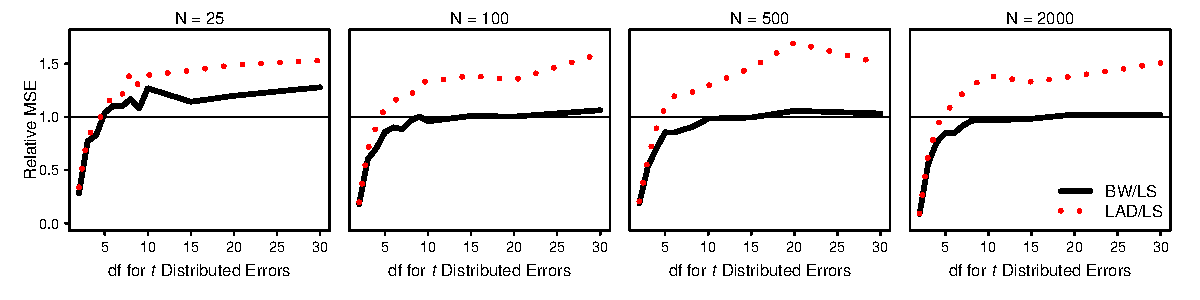
\includegraphics[width = \textwidth]{figs/mc-sims.pdf}
\caption{This figure shows the relative MSE for the LAD estimator and the BW estimator compared to the LS estimator for $t$ distributed errors as the degrees of freedom varies. 
Notice that for very heavy-tailed distributions (e.g., two to five degrees of freedom), both the LAD and the BW estimators significantly outperform the LS estimator. 
And while the performance of the LAD estimator significantly worsens as the distribution becomes more normal, the BW estimator remains comparable to the LS estimator.}\label{fig:mc-sims}
\end{center}
\end{figure}

Notice that the LAD and BW estimators perform quite well for very heavy tailed distribution (i.e., degrees of freedom from two to four), but as the tails grow lighter, the LS estimator quickly begins to outperform the LAD estimator. 
Except for all but very heavy tailed distributions, the LS estimator is considerably more efficient than the LAD estimator. 

The BW estimator, other the other hand, is a much stronger competitor for the LS estimator. 
While the LS estimator is more efficient for lighter-tailed distributions (i.e., more than ten degrees of freedom), the difference is very small except in very small samples. 
Indeed, for sample sizes of 100 or larger, the LS estimator is only about 5\% more efficient than the BW estimator \textit{at best}. 
This second simulation also suggests that the BW estimator works almost as well as the LS estimator under ideal conditions for LS estimator and considerably better across a wide range of other, substantively plausible scenarios.

\section*{Recommendation for Applied Researchers}

When using the linear model, we suggest that researchers take steps to ensure that the assumption of normal errors makes theoretical and empirical sense. 
\begin{enumerate}
	\item Initially fit the model using least squares. 
	\item As a ``robustness check,'' re-fit the model using a robust alternative, such as the biweight estimator. 
	\item If the inferences change (and even if not), carefully examine the residuals using histograms and QQ plots. Be careful to check for skewness.
	\item If the residuals are not symmetrically distributed, then consider a transformation. 
	This transformation might be critical because it allows the model to represent non-linear relationships implied by the skewness and allows the statistical model to more closely approximate the data. 
	The log-transformation has a nice substantive interpretation, so it makes sense as a first cut, especially for variables naturally bounded below by zero or one. 
	If the log-transformation over- or under-corrects the skewness, then the Box-Cox transformation should ensure that the residuals are roughly symmetric.
	\item Once the residuals are roughly symmetric, it makes sense to re-fit the model using least squares and a robust alternative. 
	Especially if the residuals appear to have heavy tails, then the robust estimator might serve as a more efficient estimator. 
	However, the robust estimator also allows for greater substantive interpretation as well, because it allows unusual cases to stand out.
	\item Always pay close attention to the residuals from each model, especially differences, as these can be especially substantively informative.
	\item To the extent that some cases seem unusual, especially in the context of the robust regression, give these cases careful review. 
	Is it possible that these unusual outcomes are simply data entry errors? 
	In light of these cases, can the measurement be improved? 
	Might a subset of the cases be operating under a substantially different causal process that could be built into the statistical model? 
\end{enumerate}

\section*{Replication of Clark and Golder (2006)}

\cite{ClarkGolder2006} attempt to ``rehabilitate'' Duverger's (\citeyear{Duverger1963}) classic explanation for the number of political parties in a system.
They write: 

\begin{quote}
According to Duverger, the mechanical effect of electoral institutions favoring large parties creates incentives for strategic entry and strategic voting. 
Parties that have no chance of winning are encouraged to withdraw. 
If these parties fail to withdraw, then voters will have an incentive to vote strategically in favor of better placed parties. 
Thus disproportional systems with low district magnitudes are likely to reduce the demand for political parties created by social heterogeneity (p. 694).
\end{quote}

For our replication, we focus specifically on their hypothesis:
\begin{quote}
\textsc{Hypothesis:} Social heterogeneity increases the number of electoral parties only when the district magnitude is sufficiently large.
\end{quote}

This suggests that the marginal effect of social heterogeneity should be positive and statistically significant under permissive electoral rules (i.e., large district magnitude) and about zero and statistically insignificant (though see Rainey 2014) under restrictive electoral rules (i.e., district magnitude near one).

To measure their key outcome variable, the number of political parties, Clark and Golder use the \textit{effective} number of political parties (ENEP), where $\text{ENEP} = \sum_{i = 1}^n\frac{1}{v_i^2}$, for $v_i$ represents the vote share of party $i$ in the election. 
Similarly, for their measure of social heterogeneity, Clark and Golder use the effective number of ethnic groups (ENEG), taken from Fearon's (2003) measure of ethnic fragmentation. 
To measure the restrictiveness of the electoral rules, Clark and Golder simply use the average district magnitude in the election. 

Figure \ref{fig:cg-scatter} plots the key explanatory variables, district magnitude and the effective number of ethnic groups, along the horizontal and vertical axes, respectively. 
The size of the points indicates the effective number of political parties for each election. 
The hypothesis predicts that the large points should lie in the upper-right section of the plot and small points should lie near the horizontal and vertical axes.

\begin{figure}[h!]
\begin{center}
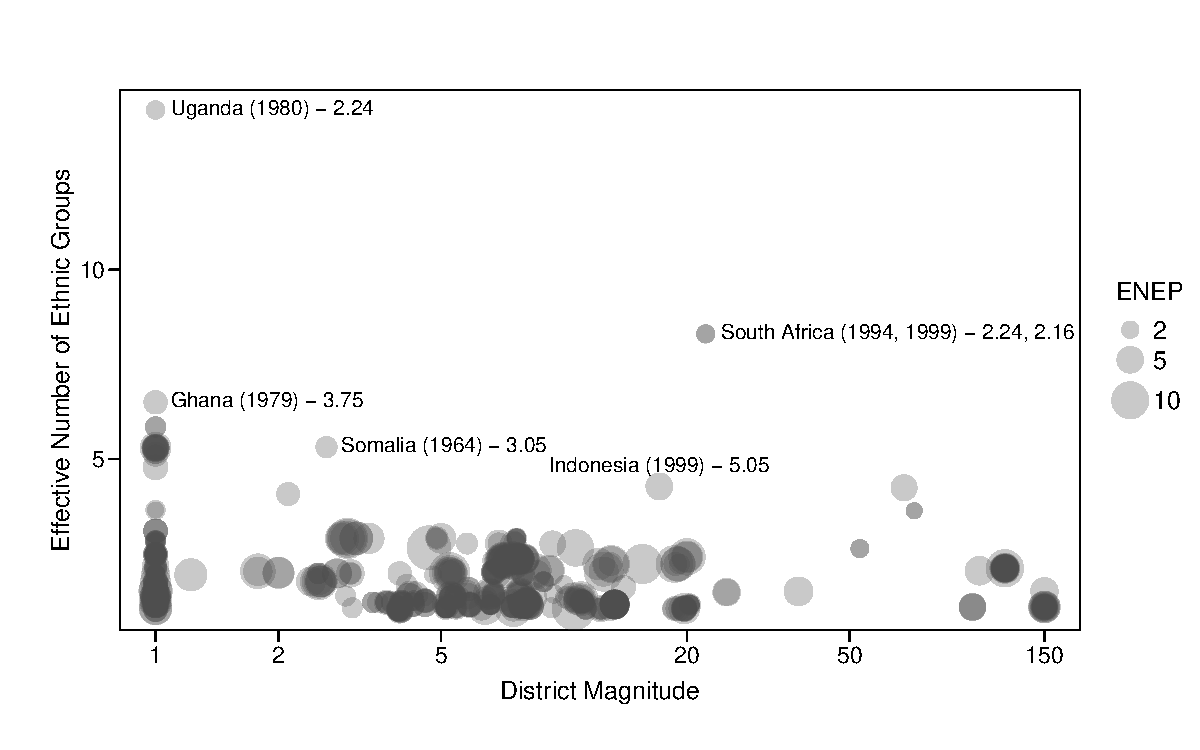
\includegraphics[scale = 0.8]{figs/cg-scatter.pdf}
\caption{This figure shows the distribution of district magnitude (on the log scale) and ethnic heterogeneity, where the point sizes indicate the number of political parties. 
According to Clark and Golder's hypothesis, large points should lie in the upper-right portion of the plot and small points should lie along the axes.}\label{fig:cg-scatter}
\end{center}
\end{figure}

To test this hypothesis, Clark and Golder fit the following linear model using least squares:
\begin{align*}
\text{ENEP}_i = \beta_0 &+ \beta_1 \text{ENEG}_i + \beta_2 \log(\text{Magntiude}_i) + \beta_3 \text{Upper-Tier Seats}_i\\
                                                     &+\beta_4 \text{Presidential Candidates}_i + \beta_5 \text{Proximity}_i\\
                                                     &+ \beta_6 \text{Ethnic}_i \times \log (\text{Magnitude}_i) + \beta_7 \text{Ethnic}_i \times \text{Upper-Tier Seats}_i\\
                                                     &+ \beta_7 \text{Presidential Candidates}_i \times \times \text{Proximity}_i + \epsilon_i\text{ ,}
\end{align*}

The first key coefficient in this analysis is $\beta_1$, which captures the effect of social heterogeneity when district magnitude is one (i.e., the log of district magnitude is zero) and there are no upper-tier seats. 
According to the hypothesis, $\beta_1$ should be about zero. 
The second key coefficient is $\beta_6$, which captures how the effect of social heterogeneity changes with the electoral rules. 
According to the hypothesis, $\beta_6$ should be positive, so that the effect of social heterogeneity becomes (perhaps more) positive as the district magnitude increases.

Clark and Golder use least squares to obtain their estimates of the model coefficients, but worry about their estimates of the standard errors. 
They write that ``[t]he crucial thing to remember is that although OLS is consistent with longitudinal data, the standard errors may be incorrect'' (p. 690). 
They discuss several options and ultimately settle on robust standard errors clustered by country, but demonstrate that their conclusions are robust to alternative approaches to estimating standard errors. 
However, they do not address the possibility of a non-normal error distribution or its potential impact on the coefficient estimates. 
This is especially concerning given that the effective number of electoral parties is bounded below by zero, perhaps creating an error distribution with a skew to the right. 

To get an initial sense of how the results might change using an alternative (perhaps more efficient) estimator, we replicated the estimates from four models in their Table 2 using least squares and the biweight estimator. 
For these initial estimates, we make no attempt to account for the clustered nature of the data in calculating the standard errors, but do supply the usual 90\% confidence intervals to serve as a lower-bound on the uncertainty. 
Figure \ref{fig:cg-coef-plots} presents these estimates and confidence intervals.

\begin{figure}[h!]
\begin{center}
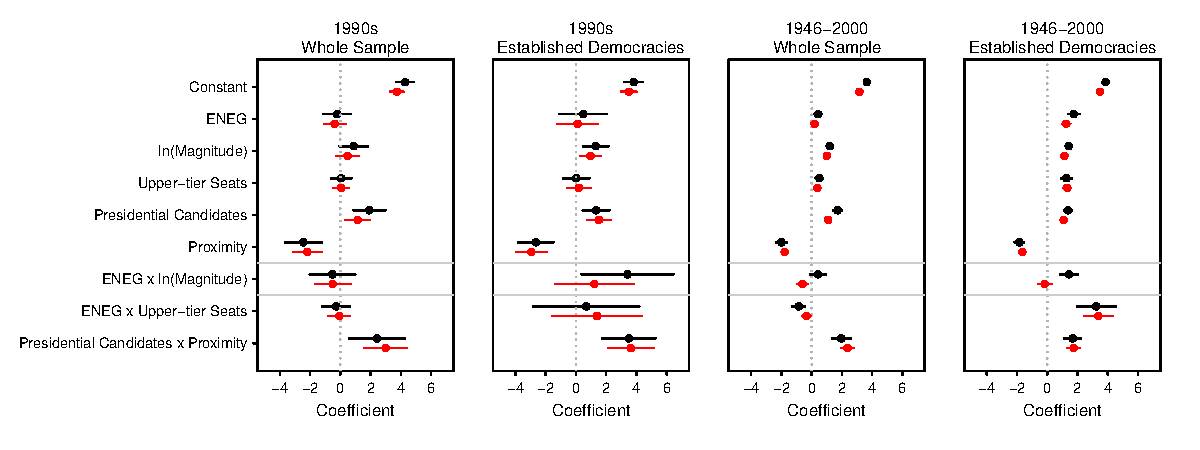
\includegraphics[scale = .8]{figs/cg-coef-plots.pdf}
\caption{This figure shows the coefficient estimates of Clark and Golder's (2006) linear model using a least-squares and biweight estimator with explanatory variables standardized to have mean zero and standard deviation one-half. 
The black lines and points show the least squares estimates and 90\% confidence intervals and the red lines and points show the biweight estimates and confidence intervals. 
Notice that the coefficient for the product of the effective number of ethnic groups and the district magnitude changes drastically with the choice of estimator.}\label{fig:cg-coef-plots}
\end{center}
\end{figure}

The crucial estimate $\hat{\beta}_6$ changes substantially depending on the choice of estimator. 
This key estimate, which the theory suggests should be positive, remains negative in the 1990s sample including new democracies, shrinks substantially toward zero in the 1990s sample that includes only established democracies, and \textit{becomes negative} in the large sample of countries from 1946-2000 that includes new democracies \textit{and} the large sample that only includes established democracies. 
When results depend on the choice of estimator, it is especially important to carefully examine the residuals.

For the remainder of our analysis, we focus on the estimates from large sample of countries from 1946-2000 that includes only established democracies. 
Figure \ref{fig:cg-residuals-hist} presents the histogram of the residuals from the least-squares estimates and Figure \ref{fig:cg-qq-plot} presents the QQ plot for these residuals. 
Both figures indicate a substantial skew to the right. 
While this does not necessarily lead to biased estimates, it does, in our view, suggest that the linear model would be more appropriate for a transformed outcome variable. 
If the transformation makes the errors more closely approximate a normal distribution, then the least squares estimators will be more efficient. 
The model for the transformed outcome can capture potentially interesting substantive effects as well.

\begin{figure}[h!]
\begin{center}
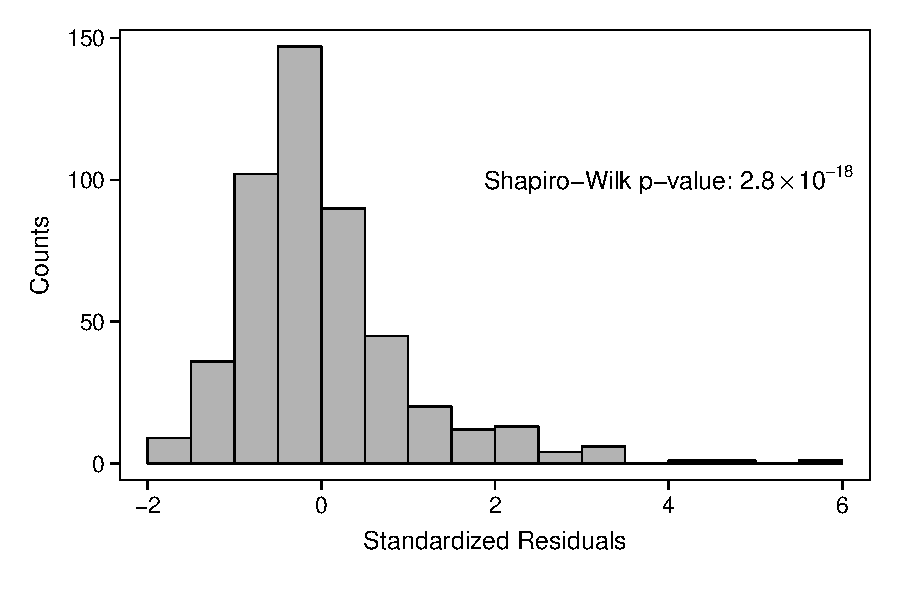
\includegraphics[scale = 0.6]{figs/cg-residuals-hist.pdf}
\caption{This histogram shows the distribution of the residuals from Clark and Golder's (2006) main model. 
Notice that these residuals do not seem approximately normal. They have a strong skew to the right. 
For example, one would rarely expect to observe residuals more that three standard deviations from zero if the assumption of normality holds. 
In these data, we have several residuals more that three standard deviations away and one nearly six standard deviations away. 
This suggests that some transformation of the outcome variable might be useful.}\label{fig:cg-residuals-hist}	
\end{center}
\end{figure}

\begin{figure}[h!]
\begin{center}
	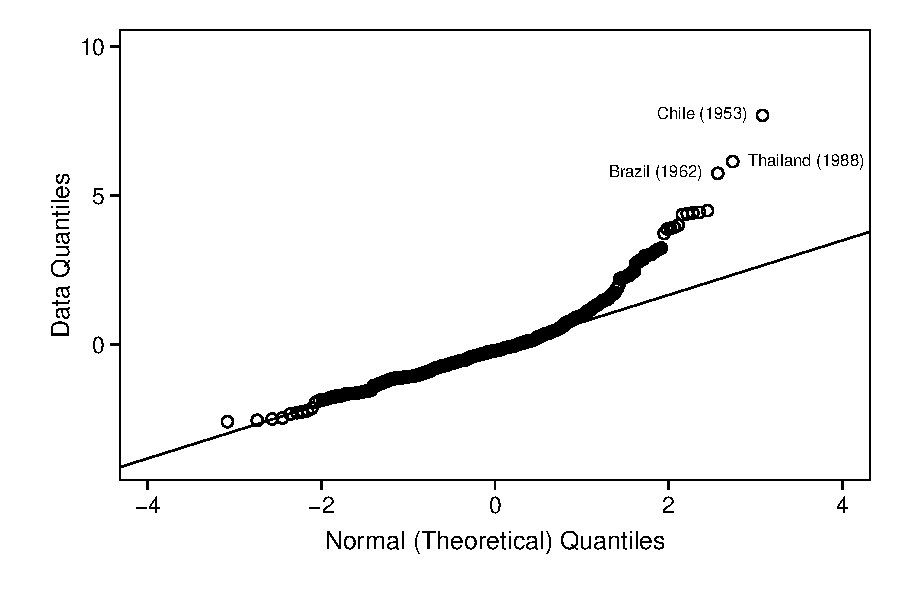
\includegraphics[scale = 0.6]{figs/cg-qq-plot.pdf}
\caption{This QQ plot shows the deviation of the residuals from normality in Clark and Golder's (2006) main model. 
If the residuals were approximately normal, then the points in the QQ plot would approximately follow the line. 
However, notice that the positive residuals deviate sharply from the theoretical expectations. 
This also suggests that some transformation of the outcome variable might be useful.}\label{fig:cg-qq-plot}
\end{center}

\end{figure}

The maximum likelihood estimate of the Box-Cox transformation parameter $\lambda$ is about $-\frac{1}{3}$ and the confidence interval does not include zero, which suggests that a log-transformation does not quite eliminate the skew. 
We re-estimated the model using both a log-transformation and Box-Cox transformation with $\lambda = -\frac{1}{3}$. 
Figure \ref{fig:cg-trans-residuals-hist} presents the histograms of the residuals from these two regression models. 
Notice that log-transforming the effective number of electoral parties does not quite eliminate the skew in the residuals. However, the Box-Cox transformation with $\lambda = -\frac{1}{3}$ produces highly symmetric residuals. 

\begin{figure}[h!]
\begin{center}
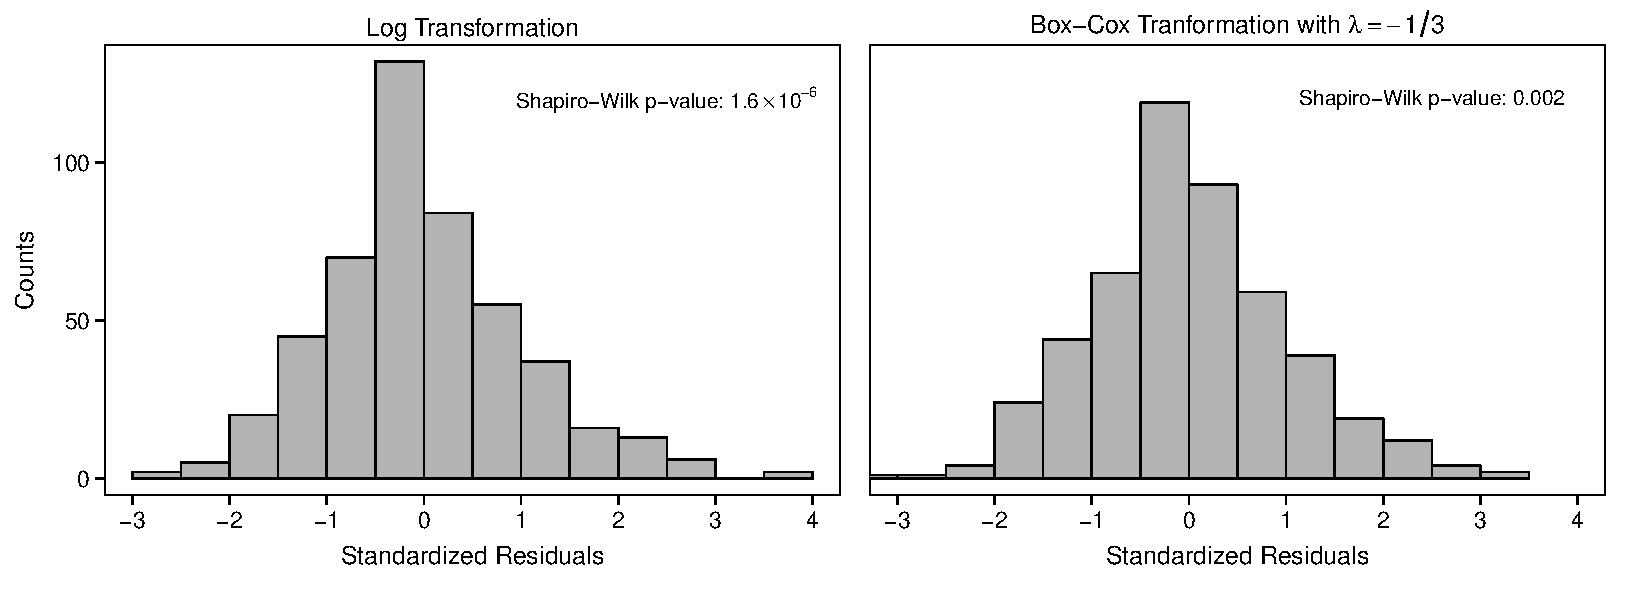
\includegraphics[width = \textwidth]{figs/cg-trans-residuals-hist.pdf}
\caption{These histograms shows the distribution the residuals after transforming the outcome variable. 
The left panel shows that the log transformation does not quite remove all of the skew, but the right panel shows that the Box-Cox transformation with $\lambda = -\frac{1}{3}$ creates an approximately symmetric error distribution.}\label{fig:cg-trans-residuals-hist}
\end{center}
\end{figure}

Figure \ref{fig:cg-trans-qq-plot} shows the QQ plot for the residuals. 
The left panel confirms that a right-skew remains after the log-transformation, as suggested by the histogram in the left panel of Figure \ref{fig:cg-trans-residuals-hist}. 
The right panel of Figure \ref{fig:cg-trans-qq-plot} confirms that the Box-Cox transformation removes much or all of this skew, as suggested by the right panel of Figure \ref{fig:cg-trans-residuals-hist}. 

\begin{figure}[h!]
\begin{center}
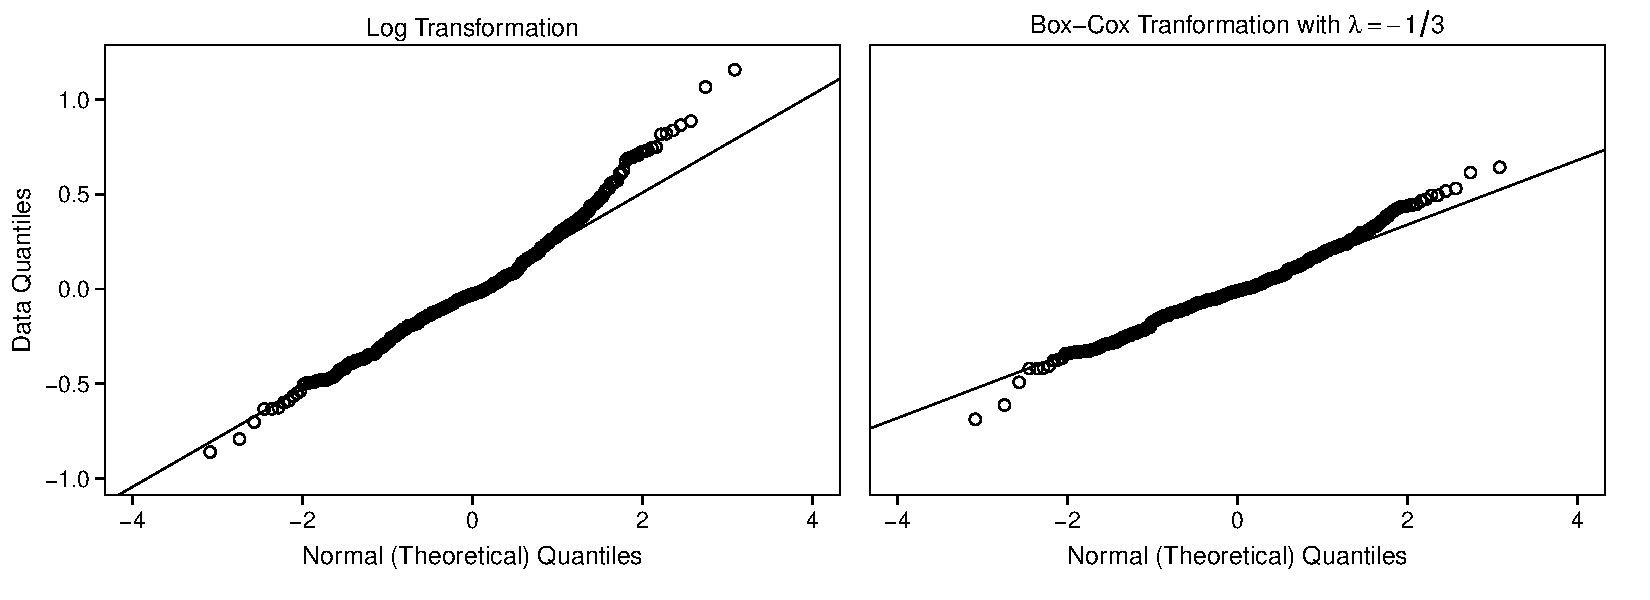
\includegraphics[width = \textwidth]{figs/cg-trans-qq-plot.pdf}
\caption{These QQ plots show residuals after transforming the outcome variable.
The left panel shows that the log transformation does not quite remove all of the skew, but the right panel shows that the Box-Cox transformation with $\lambda = -\frac{1}{3}$ creates an approximately symmetric error distribution, though it has heavier tails than a normal distribution.}\label{fig:cg-trans-qq-plot}
\end{center}
\end{figure}

Although the Box-Cox transformation removes much or all of the skew, the residuals retain tails that are slightly heavier than the tails of the normal distribution. 
The residuals have larger positive and negative quantiles than one would expect under a normal distribution. 
This suggests the residuals follow a heavy-tailed distribution, perhaps resembling a $t$ distribution with degrees of freedom in the range of six to twelve. 
Even after the Box-Cox transformation, the Shapiro-Wilk test rejects the null hypothesis of normality with $p = 0.002$. 
Assuming that these residuals follow a $t$-distribution, we can estimate the degrees of freedom using maximum likelihood estimate, which points toward a $t$ distribution with about ten degrees of freedom. 
Recall that the biweight estimator is a (slightly) more efficient estimator for $t_{10}$ distributed errors. 
However, the least squares estimates \textit{assumes} normally distributed errors and thus the error distribution might have \textit{even heavier} tails.

Most importantly, after the Box-Cox transformation, the residuals are well-behaved. 
They are highly symmetric and only slightly heavy-tailed. 
In spite of nearly ideal situation, the simulations in Tables \ref{tab:mc-sims-100} and \ref{tab:mc-sims-1000} and Figure \ref{fig:mc-sims} suggest that the biweight estimate is a slightly better estimator. 
But these differences are slight so it can be valuable to carefully examine examine both models---one that tries to fit all the data well and another that tries to fit most of the data well.

\subsection*{Quantities of Interest}

To estimate the quantity of interest---the effect of social heterogeneity as the permissiveness of the electoral rules varies---we re-estimated Clark and Golder's model with and without the Box-Cox transformation using both the least squares and biweight estimators. 
To obtain standard errors, we using the cluster bootstrap suggested by \cite{Harden2012} to calculate the confidence intervals for each model.

Figure \ref{fig:cg-fd-plots} plots the effect of increasing social heterogeneity from ENEP = 1.06 (10th percentile) to ENEP = 2.48 (90th percentile) as the district magnitude varies. 
The upper-left figure replicates Clark and Golder's approach (except for the cluster-bootstrap confidence intervals) and replicates their finding, which they summarize:

\begin{quote}
[These results] clearly illustrate that in established democracies, ethnic heterogeneity significantly increases the number of parties once the electoral system is sufficiently permissive. 
This is exactly what Duverger's theory predicts. 
To be more specific, Figure 1a [our upper-left panel of Figure \ref{fig:cg-fd-plots}], based on the pooled model with established democracies, indicates that ethnic heterogeneity will increase the number of electoral parties once we move beyond nonpermissive electoral systems with single-member districts when [Magnitude = 1].
\end{quote}

\begin{figure}[h!]
\begin{center}
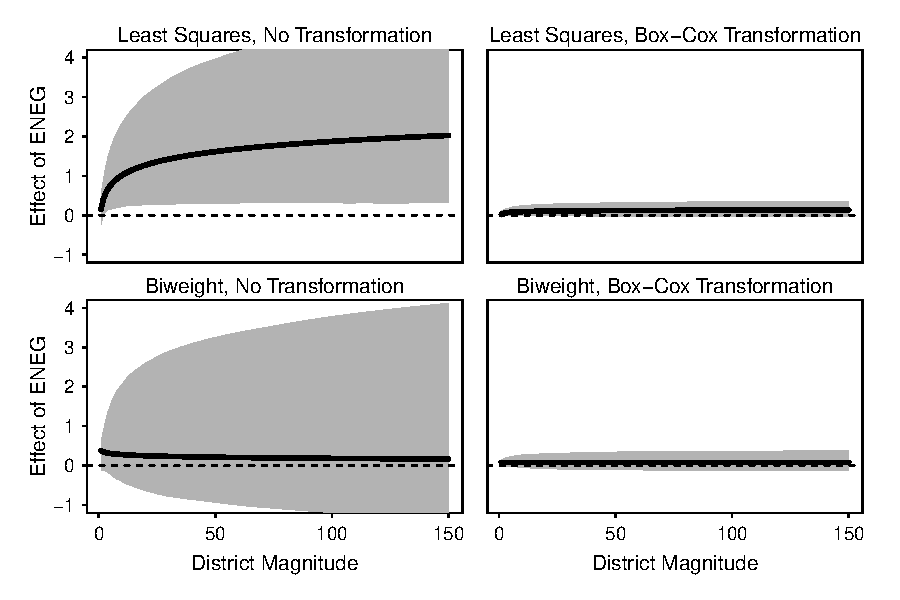
\includegraphics[width = \textwidth]{figs/cg-fd-plots.pdf}
\caption{This figures shows the estimated effects and 90\% confidence intervals of increasing social heterogeneity from ENEP = 1.06 (10th percentile) to ENEP = 2.48 (90th percentile) on the effective number of electoral parties as the district magnitude varies. 
Notice that only the model that does not use robust estimators or transform the outcome variable provides evidence in support of the hypothesis.}\label{fig:cg-fd-plots}
\end{center}
\end{figure}

But this evidence breaks down once we adjust for the non-normality of the errors. 
The lower-left panel of Figure \ref{fig:cg-fd-plots} shows that simply using the biweight estimator as a robust alternative to least squares produces estimated interaction in the \text{opposite} direction as the hypothesis predicts, though small and not statistically significant. 
The upper-right panel of Figure \ref{fig:cg-fd-plots} shows that simply transforming the outcome variable to make the data more consistent with the assumed normal-linear model substantially increases the uncertainty across the range of district magnitude, so that small negative effects are now plausible, as well as much larger positive effects. 

However, we argue that the best approach for these data is to transform the outcome variable to obtain a roughly symmetric error distribution \textit{and} use the biweight estimator to handle the remaining heavy tails shown in the left panel of Figure \ref{fig:cg-trans-qq-plot}. 
This approach reduces effect of social heterogeneity somewhat across the range of district magnitude.

Because the scale of the estimates and uncertain differ drastically across the choice to transform the outcome variable or not, as well as the range of district magnitude, we present the relevant quantities of interest in Table \ref{tab:cg-qi}. 
In this case, we are interested in the effect of substantially increasing social heterogeneity from ENEP = 1.06 (10th percentile) to ENEP = 2.48 (90th percentile) on the number of political parties when district magnitude is one (10th percentile) and also when district magnitude is 14 (90th percentile). 
Since the hypothesis suggests that this effect should be larger when the district magnitude is larger, we are also interested in the difference between these two effects. 
For simplicity, we simply focus our discussion on the differences between the typical approach, least squares with no transformation, and the approach we recommend, transformation \textit{and} robust estimation.

The first row of Table \ref{tab:cg-qi} suggests that in countries with single-member districts, a substantial increase in ENEG (10th to 90th percentile) increases the ENEP by about 0.16 [-0.24; 0.53] parties. 
On the other hand, in large, multimember districts (magnitude of 14), the same increase in social heterogeneity increases the ENEP by about 1.14 [0.26; 2.67] parties. 
This is just as the hypothesis predicts. 
Further, this increase of 0.98 [0.06; 2.65] is large and statistically significant.\footnote{Using cluster-robust standard errors, Clark and Golder find that the product term is \textit{not quite} significant. We use cluster-bootstrap standard errors and find the the coefficient is \textit{barely} significant.}

\begin{table}[h!]
{\scriptsize
% quantreg::latex.table(x = qitab, file = "doc/tabs/cg-qi", rowlabel = "",      rowlabel.just = "l", cgroup = c("First-Difference When \\textit{M} = 1",          "First-Difference When \\textit{M} = 14", "Second-Difference"),      rgroup = c("No Transformation", "Box-Cox Transformation"),      n.rgroup = c(2, 2), table.env = FALSE) 
%
\begin{center}
\begin{tabular}{|l||c|c||c|c||c|c|} \hline
\multicolumn{1}{|l||}{\bf }&\multicolumn{2}{c||}{\bf First-Difference When \textit{M} = 1}&\multicolumn{2}{c||}{\bf First-Difference When \textit{M} = 14}&\multicolumn{2}{c|}{\bf Second-Difference}\\ \cline{2-7}
\multicolumn{1}{|l||}{}&\multicolumn{1}{c|}{Est.}&\multicolumn{1}{c||}{90\% CI}&\multicolumn{1}{c|}{Est.}&\multicolumn{1}{c||}{90\% CI}&\multicolumn{1}{c|}{Est.}&\multicolumn{1}{c|}{90\% CI}\\ \hline
{\bf No Transformation}&&&&&&\\
~~Least Squares&~~~~~0.16~~~~~&[-0.24;~~0.53]&~~~~~1.14~~~~~&[0.26;~2.67]~~&~~~~~0.98~~~~~&[0.06;~2.65]~~\\ 
~~Biweight&~~~~~0.37~~~~~&[-0.12;~~0.62]&~~~~~0.26~~~~~&[-0.51;~~2.33]&~~~~~-0.11~~~~&[-0.96;~~2.05]\\ \hline
{\bf Box-Cox Transformation}&&&&&&\\
~~Least Squares&~~~~~0.03~~~~~&[-0.05;~~0.12]&~~~~~0.10~~~~~&[0.00;~0.26]~~&~~~~~0.07~~~~~&[-0.07;~~0.26]\\ 
~~Biweight&~~~~~0.08~~~~~&[-0.04;~~0.15]&~~~~~0.08~~~~~&[-0.06;~~0.28]&~~~~~0.00~~~~~&[-0.17;~~0.25]\\ 
\hline
\end{tabular}
\end{center}

}
\caption{This table shows the quantities of interest from least squares and biweight estimates, with and without the Box-Cox transformation of the outcome variable. 
Notice that the least squares estimates without transforming the outcome variable are consistent with Clark and Golder's hypothesis. 
However, transforming the outcome variable, using the robust biweight estimator,  or both substantially reduces the amount of evidence that these data offer in favor of the hypothesis.}\label{tab:cg-qi}
\end{table}

However, once we make an effort to account for the non-normality of the residuals by transforming the outcome variable \textit{and} using the robust biweight estimator, this evidence for interaction weakens slightly. 
This model suggests that, in single-member districts, a substantial increase in social heterogeneity increases the ENEP by about 0.29 [-0.13; 0.48] parties. 
This is about twice Clark and Golder's initial estimate.
In large, multimember districts (magnitude of 14), the estimate shrinks to 0.62 [-0.41; 3.34], which is about half of Clark and Golder's estimate. 
This leads to an estimated increase of 0.33 [-0.78; 3.14] in the effect of social heterogeneity as we move from single-member districts to large, multimember districts---about one-third of Clark and Golder's initial estimate.

\subsection*{Differences Between the Estimates}

One major advantage of redescending estimators, such as the biweight estimator, is that these estimators allow unusual cases to stand out. 
Figure \ref{fig:cg-residuals-compare} compares the residuals from the least squares fit and the biweight fit after the Box-Cox transformation. 
Notice that the residuals tend to agree, with the exception of the 1980 election in Uganda, which is the largest residual in the biweight fit, but does not stand out among the least squares residuals.

\begin{figure}[h!]
\begin{center}
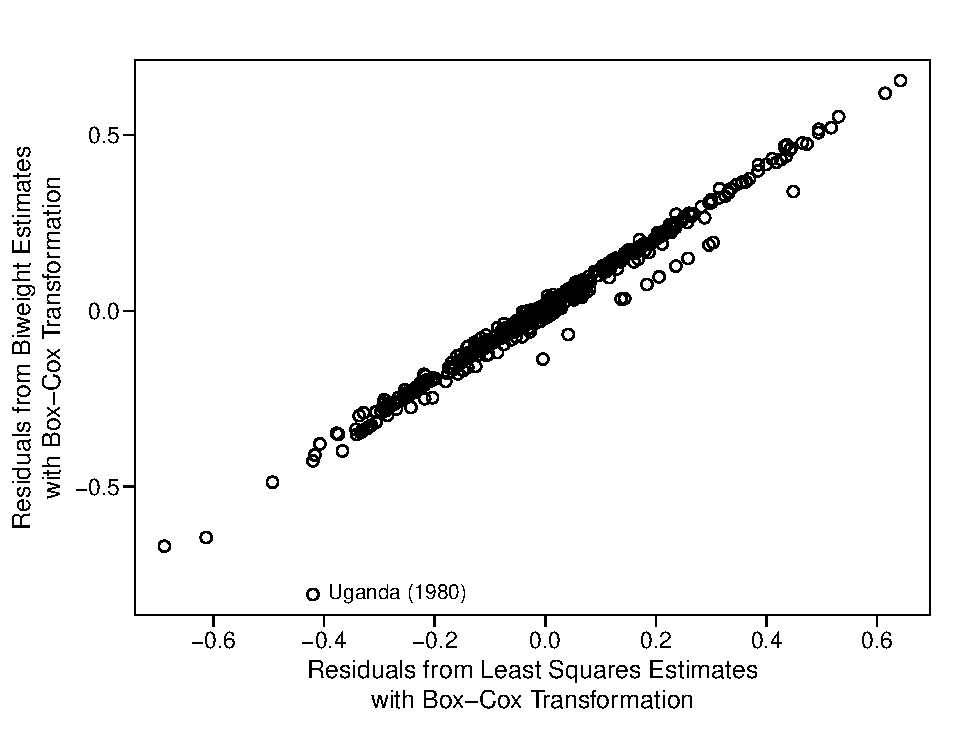
\includegraphics[scale = 0.6]{figs/cg-residuals-compare.pdf}
\caption{This figure shows the relationship between the least squares and biweight estimates after the Box-Cox transformation. 
Notice that the biweight estimate allows the unusual case of Uganda to stand out from the others.}\label{fig:cg-residuals-compare}
\end{center}
\end{figure}

Similarly, Figure \ref{fig:cg-weights} presents the 35 smallest weights from the biweight fit. 
Recall that as cases become increasingly inconsistent with the majority of the data, the biweight estimator increasingly down weights these cases, potentially to zero. 
As we might expect, given the residuals in Figure \ref{fig:cg-residuals-compare}, the 1980 election in Uganda receives zero weight. 
This election is consistent with the hypothesis because it features single member districts, an extremely large number of ethnic groups, and only two major political parties. 
Unfortunately for the hypothesis, though, this case is inconsistent the the majority of the data.

\begin{figure}[h!]
\begin{center}
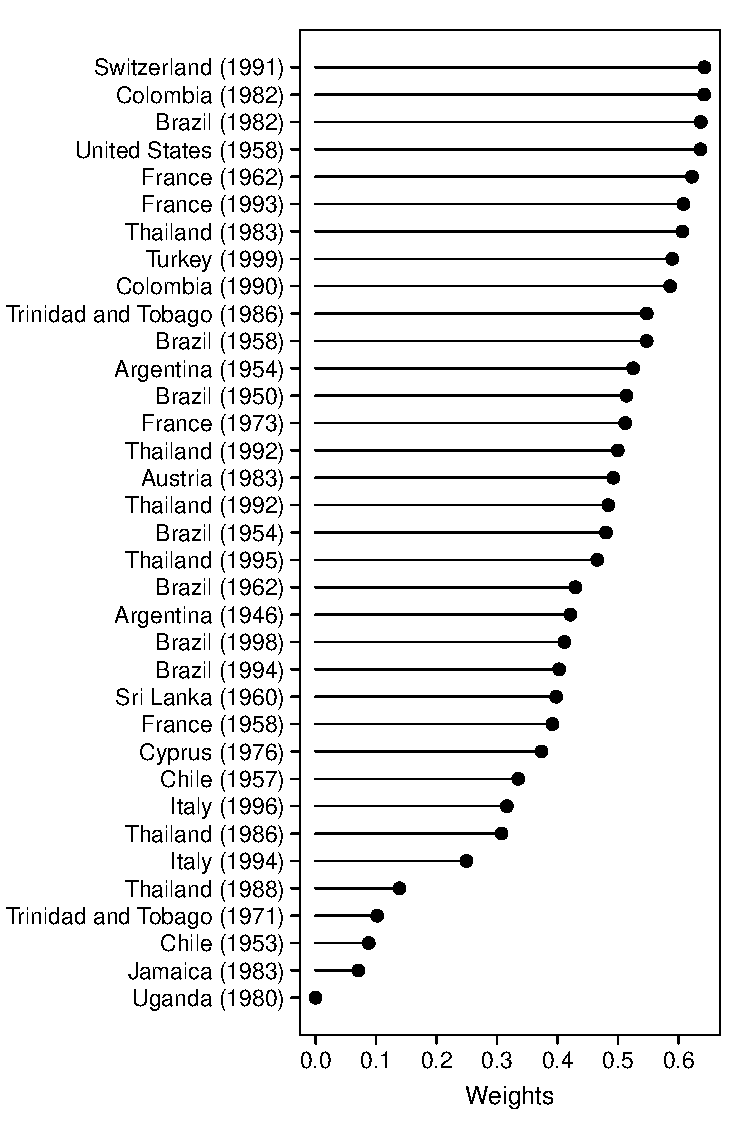
\includegraphics[scale = 0.7]{figs/cg-weights.pdf}
\caption{This figure shows the final weights implied by the biweight estimator. 
Because the 1980 election in Uganda is quite different from the remainder of the data, the biweight estimator downweights this case all the way to zero.}\label{fig:cg-weights}
\end{center}
\end{figure}

\subsection*{Some Implications the Results}

We offer a different approach than most applied research in political science adopts in practice. 
Rather than relying on the artificial Gauss-Markov theorem and BLUE estimators, we suggest that a careful consideration of the residuals is important. 
We have shown that there can be tremendous gains in efficiency by using robust estimators in the face of heavy-tailed error distributions, and we have shown that our approach leads to somewhat different conclusions than \cite{ClarkGolder2006}. 
But the approach we advocate is not powerful because it gives different results---it is powerful because it is substantively informative. 
Below we discuss several \textit{substantive} points that one can take from our brief analysis of Clark and Golder's data.

\subsubsection*{Questions about the Validity of the Theory}

At first glance, these results might make it seem Duverger's logic lacks the empirical support suggested by the literature. Indeed, the evidence offered by the normal-linear model seems to hinge on the improper assumption of normal errors. 
Once we relax this assumption using a transformation and robust estimators, the evidence shrinks. However, rejection of Duverger's theory or Clark and Golder's (2006) analysis is premature for four reasons. 
First, the theoretical logic for Duverger's hypotheses is clear and compelling (e.g., \citealt{Duverger1963}, \citealt{Riker1982}, \citealt{Cox1997}, \citealt{AmorimNetoCox1997}, \citealt{Cox1999}). 
Second, many empirical studies beyond \cite{ClarkGolder2006} find substantial empirical support for the hypotheses, including observational (e.g., \citealt{ChhibberKollman1998} and \citealt{SingerStephenson2009}, quasi-experimental (e.g., \citealt{Blaisetal2011} and \citealt{Fujiwara2011}), and incentivized experimental studies (for a review, see \citealt{Rietz2008}). 
Thirdly, in addition to the confidence intervals including effects that are inconsistent with the Clark and Golder's hypothesis, the confidence intervals now include \textit{even larger} effects, which suggests the effect might be even larger than Clark and Golder suggest.
Finally, the biweight $M$-estimator suggests several potential shortcomings in terms of concepts, theory, measurement that might currently undermine the evidence for these theories.

\subsubsection*{Questions about Measuring ``Established Democracies''}

These results suggest we have room for improvement in our measurement of ``established democracies.'' 
Figure \ref{fig:cg-weights} suggests that the 1980 election in Uganda is quite different from the remaining cases, so we might look more closely at the context of the election.
Uganda was under British rule until 1962, when it was granted independence from Britain. 
The 1962 elections led to the election of Milton Obote as prime minister. 
Four years later, facing scandal, Obote suspended the constitution, assumed all government powers, and declared himself president. 
In 1967, the parliament adopted a new constitution that solidified the expansive powers in the hands of the president. 
During this time Obote banned all political parties and organizations accept his own \citep[p. 99]{Kasozi1993}. 
In 1971, Obote was ousted by Major General Idi Amin. During Amin's rule, between 50,000 and 300,000 civilians were killed \citep[p. 104]{Kasozi1993}. 
With the support of the Tanzanian military, which was working in conjunction with two Ugandan factions one lead by Obote and the other Museveni, ended Amin's bloody rule in 1979 (\citealt[p. 53]{Kasfir1998}, and \citealt[pp. 124-127]{Kasozi1993}).
In the following year, one leader was forcibly removed from office and the following government experience yet another military coup and elections were scheduled in 1980. 
By May of 1980, a group known as The Military Commission had taken power in order to give it to Obote. 
Obote wanted the appearance of being a democratic leader, therefore the Military Commission drafted electoral rules and held an election later that year \citep[pp. 135-137]{Kasozi1993}.
In an election that fraught with corruption and irregularity, Obote's party won a majority of the seats---this 1980 Ugandan election is this is the unusual case in the data set.
Amin's bloody rule continued into Obote's second tenure with a death toll between 100,000 and 500,000 over the next five years---a second conflict with civilian casualties on the scale of the recent tragedies in Darfur. 
Although elections were again held in 1996, 2001, 2006, and 2011, these election featured irregularities, harassment, and did not lead to a change in power.

The context of the election raises question about whether Uganda was an ``established democracy'' in 1980, or even a democracy. 
One common measure offered by \cite{CheibubGandhiVreeland2010}, does indeed code Uganda as a democracy in 1980.\footnote{Another common measure of democracy, Polity IV, codes Uganda as a four in 1980, which falls outside range of six to ten that scholars typically consider democratic.} 
They code countries as a democracy if and only if it meets all following four conditions:
\begin{enumerate}
\item The chief executive must be chosen by popular election or by a body that was itself popularly elected.
\item The legislature must be popularly elected.
\item There must be more than one party competing in the elections.
\item An alternation in power under electoral rules identical to the ones that brought the incumbent to office must have taken place.
\end{enumerate}

Although the election showed signs of irregularities and harassment of voters and candidates, it is plausible that Uganda in 1980 meets the first three criteria. 
But what about the forth? 
Because these author indeed code Uganda in 1980 as a democracy, they consider this condition met. 
However, this was a single election, nested between two military dictatorships, and during the winner's administration, he seized powers and dragged the country into civil war. 
It remains unclear to us how this meets the condition of democracy more broadly or the alternation condition more specifically.

Indeed it is becoming common for authoritarian leaders to hold meaningless elections in to present the illusion of democracy. \cite{LevitskyWay2002} argue that:
\begin{quote}
It is essential, however, to distinguish regimes in which democratic institutions offer an important channel through which the opposition may seek power from those regimes in which democratic rules simply serve as to legitimate an existing autocratic leadership.
\end{quote}

Secondly, even if Uganda was a democracy in 1980, was it ``established''? 
Surely not, as this was the first election in 18 years following 10 years of brutal dictatorship. 
However, according to Clark and Golder's define ``established democracies'' as countries that transitioned to democracy after 1989 (see note b in their Tables 1 and 2). 
Yet why is it important to focus on \textit{established} democracies? \citet[p. 706]{ClarkGolder2006} summarize Duverger's argument: 

\begin{quote}
Another intriguing finding is that Duverger's theory receives much weaker support when we include elections from countries that transitioned to democracy after 1989. 
This finding is perhaps understandable if we think that party systems in newly democratic countries take a while to reach their equilibrium. 
It is interesting that Duverger himself took this view in regard to the fledgling democracies of Central Europe, Latin America, and Africa earlier in the 20th century. 
By warning about the danger of confusing multipartism with the absence of (fully institutionalized) parties, Duverger was indicating that he did not expect his theory to work particularly well in new democracies. 
\end{quote}

This suggests some rethinking of the concept of ``\textit{established} democracy'' might be in order, at least in the context of Duverger's theory. 
For example, it surely must be the case that countries transitioning to democracy before 1989 (e.g., Uganda in 1980) are ``established'' immediately after transitioning to democracy. 
As Clark and Golder explain, the hypothesis assumes that the party system has reached an equilibrium. If systems that have not yet reached an equilibrium are included in the analysis, then we can expect the data to offer little support for the hypothesis. 
Perhaps with some rethinking of how this equilibrium is reached, we can find a better measure that indicates when systems (are likely to) reach an equilibrium.

%\subsubsection*{Questions About Measuring ``Social Heterogeneity''} (see Stoll 2009, Sellway 2011, Posner 2004)
%\textit{Room for improvement exists in the measurement of ``social heterogeneity.''}

\subsubsection*{Questions about Dynamics Prior to Equilibrium}

In order to judge when systems are likely to be in an equilibrium, we need a stronger theory about the dynamics with which systems reach an equilibrium number of parties. Duverger's logic offers a compelling explanation for the number of political parties \textit{in equilibrium}, but this tells us little about the number of political parties prior to reaching an equilibrium or the dynamics that lead to an equilibrium. 
A theory about the dynamics to reaching an equilibrium is crucial to measuring whether a party system has reach equilibrium, which, in turn, is crucial to testing Duverger's theory. 
Perhaps new democracies begin with many parties and the number shrinks until equilibrium. 
Perhaps they begin with few and the number grows until equilibrium. 
Perhaps it depends on the context. 
Some work has been done in this area (e.g.,  \citealt{Moser1999}, \citealt{CrispOlivelloPotter2012}, and \citealt{Ferrara2011}), but expanded the theoretical and empirical research in this area is crucial in its on right and for studying the number of parties in equilibrium. 

The fact that the 1980 election in Uganda featured essentially two political parties is quite interested. 
Indeed, given the social heterogeneity, we would expect many more political parties--- more than eight according to the biweight estimate and more than four according to the least squares estimate. 
Indeed, this case is so different from the majority rest of the data that it receives zero weight in the biweight estimator. 
But why? 
One potential explanation might rely on the fact that Milton Obote, elected 18 years prior before he seized power, had returned. 
The people were quite familiar with Obote. 
Perhaps this enables groups to coordinate in support of or in oppositions to Obote. 
It is difficult to know without a thorough analysis, but our analysis is suggestive that the dynamics toward an equilibrium number of parties might depend on the nature of the prior regime. 
When parties representing the prior authoritarian regime participate in the election, perhaps this helps solve the coordination problem. 
One the other hand, when the prior regime does not participate in the elections, perhaps this makes coordination difficult. 
The point is not to answer this question but to highlight that a careful consideration of the residuals along with an estimation approach that allows unusual cases to be unusual encourages the researcher to raise these types of questions.

\section*{Conclusion}

In this paper, we adopt and defend a skeptical perspective toward least squares and explain the importance of carefully scrutinizing residuals.
We first note that the restriction to linear estimators, as required by the Gauss-Markov theorem, is unnecessary, artificial, and counterproductive. 
When the errors do not follow a normal distribution, restricting ourselves to linear estimators limits our ability to efficiently estimate the model coefficients. And as \cite{BerryFeldman1985} note, the assumption of normal errors is usually difficult to defend using either theory or data. 

Secondly, we used Monte Carlo simulations to show that our preferred estimator, an $M$-estimator with a biweight objective function, performed almost as well as least squares for normal errors, slightly better than least squares for small deviations from normality, and much better than least squares for large deviations from normality. 
In our view, political scientists should prefer this robust behavior to the more fragile least squares estimator.

Thirdly, we used a practical example to show that a more robust estimator can \textit{constructively} alter substantive conclusions. 
Robust estimators not only more efficiently estimate the model coefficient under deviations from normality, but perhaps more importantly, allow usual cases to stand out as usual. 
This, in turn, allows researchers to identify and investigate these cases carefully and improve the theoretical model, the statistical model specification, and/or the measurement of the concepts.

\singlespace
\bibliographystyle{apsr_fs}
\bibliography{/Users/carlislerainey/Dropbox/papers/bibliography/bibliography.bib}

\end{document}
